
\chapter{Návrh snímacieho systému} 
\label{kap:návrh systému}
\pagestyle{fancy}
\fancyhf{}
\fancyfoot[CE,CO]{\thepage}
\renewcommand{\footrulewidth}{1pt}
\lhead{Návrh snímacieho systému}

Pre návrh algoritmu, ktorý umožní vytvorenie precízneho modelu dynamického objektu, je potrebné navrhnúť vhodný kamerový systém. Práve špecifická aplikácia systému môže výrazne ovplyvniť možnosti skenovania. Snímaný objekt je zastúpený pediatrickým pacientom. Jeho povrchová štruktúra nie je pevná a v čase sa môže meniť. Tento fakt môže ovplyvniť geometrickú presnosť modelu hlavne ak je dĺžka doby skenovania príliš dlhá. Cieľom tejto kapitoly je overiť a navrhnúť možnosti snímania pediatrických pacientov.

%\section{Výber kamier}

%\subsection{Intel Realsense SR300}
%
%Táto kamera pracuje na princípe SLS a predstavuje vylepšenú verziu staršej Intel RealSense F200. Ide o cenovo dostupnú hĺbkovú kameru, ktorá sníma hĺbku v rozsahu od $0.2-1.5 m$. Poskytuje dynamické snímanie scény pri nízkej spotrebe (napájanie cez USB). V kombinácií s farebným obrazom ($1920\times1080p$, $30Hz$) a hĺbkovou mapou ($640x480p$) ide o jednu z najlepších dostupných SLS kamier na trhu. 
%
%\begin{figure}[H]
%	\centering
%	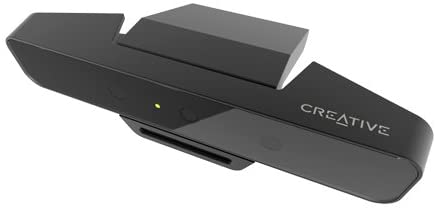
\includegraphics[width=0.7\textwidth]{figures/sr300.jpg}
%	\caption{SLS kamera Intel RealSense SR300.}
%	\label{fig::sr300}
%\end{figure}
%
%Táto kamera obsahuje RGB senzor, IR laserový projektor, IR prijímač a mikrofón. Detailnejšie opísanie princípu SLS je v podkapitole \ref{sec:sls}.

\section{Microsoft Kinect v2}

Ide o druhú generáciu hĺbkových kamier od spoločnosti Microsoft. Oproti prvej generácii využíva technológiu ToF (detailnejšie v \ref{sec:tof}), pričom ide o jednu z najznámejších senzorov tohto typu na svete \cite{wiki:kinect}. Rozsah snímanej scény je $0.5-4.5 m$. Farebný obraz je dodávaný v rozlíšení $1920\times1080p$ a $30Hz$, hĺbková mapa ma rozlíšenie $512\times424$.

\begin{figure}[H]
	\centering
	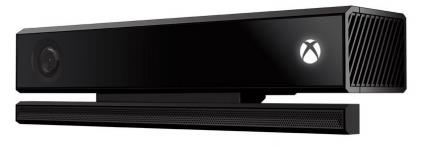
\includegraphics[width=0.7\textwidth]{figures/kinect.png}
	\caption{ToF kamera Microsoft Kinect v2 \cite{sekelova}.}
	\label{fig::kinect}
\end{figure}

Presnosť hĺbkovej mapy je oproti prvej verzii Kinectu vyššia, taktiež je znížený negatívny vplyv spôsobený slnečným svetlom.


%\subsection{Porovnanie presnosti kamier}
%
%Cieľom testovania bolo porovnať presnosť 3D rekonštrukcie statického objektu pre kamery Intel RealSense SR300 a Microsoft Kinect v2. Pomocou programov, určených k práci s jednotlivými kamerami, bola vytvorená séria snímok hĺbkových máp a ich rekonštruovaných 3D modelov. Pred snímaním bola vykonaná geometrická kalibrácia kamier, ktorej technické detaily sú opísané v kapitole \ref{sec:kinect_calib}. Kalibrovanými kamerami sa následne z 3 uhlov (pohľady spredu, z ľavej a pravej strany) získali ich 3D rekonštrukcie, ktoré zachytávali všetky potrebné detaily pre meranie. Identické natočenie pre obe kamery bolo zabezpečené rotačným podstavcom. 
%
%\begin{figure}[H]
%	\centering
%	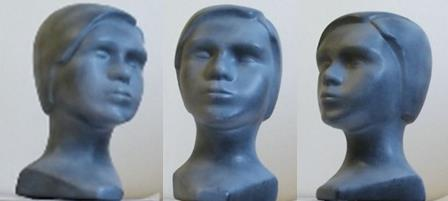
\includegraphics[width=0.7\textwidth]{figures/rgb_compar.png}
%	\caption{ToF kamera Microsoft Kinect v2.}
%	\label{fig::rgb_compare}
%\end{figure}
%
%Povrch objektu bol špeciálne upravený, aby nevytváral odlesky spôsobujúce zhoršovanie rekonštruovaného 3D modelu. 

\section{Snímanie dynamických objektov}

Pri snímaní dynamických objektov je potrebné uvažovať so vznikom pohybových artefaktov. Tie vznikajú, ak objekt v dobe skenovania mení svoje priestorové umiestnenie. Z toho dôvodu je potrebné buď stabilizovať objekt počas doby snímania alebo redukovať časovú dĺžku skenovania. Keďže tento systém má byť určený pre medicínske aplikácie, kde skenovaný objekt bude pediatrický pacient, je potrebné overiť možnosti experimentálne.


\subsection{Jedno-kamerové snímanie dynamických objektov}

Experimentálne snímanie pacientov bolo vykonávané na Klinike detí a dorastu Jesseniovej lekárskej fakulty v Martine, Laboratórium spánkovej medicíny. Do testu bolo vybraných 9 pacientov rôzneho pohlavia, vo vekovom rozmedzí od 4 do 12 rokov. Ako skenovací nástroj bola použitá kamera Kinect v2.

\begin{figure}[h]
	\centering
	\begin{subfigure}[b]{\textwidth}
		\centering
		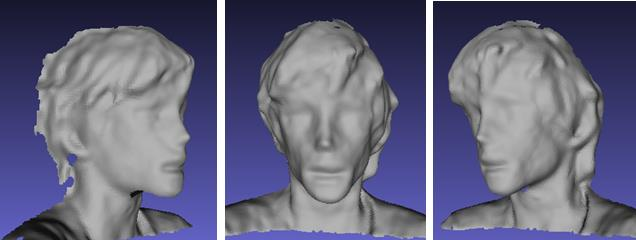
\includegraphics[width=0.8\textwidth]{figures/dynamic_patient_a.png}
		\label{fig:dynamic_patient:a}
	\end{subfigure}
	\vskip 8pt 
	\begin{subfigure}[b]{\textwidth}
		\centering
		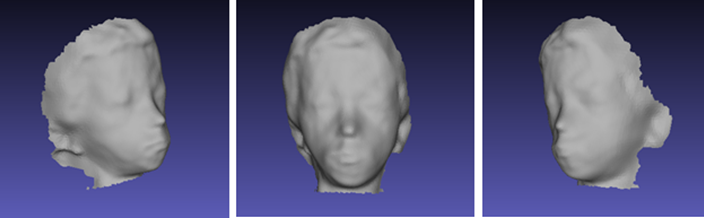
\includegraphics[width=0.8\textwidth]{figures/dynamic_patient_b.png}
		\label{fig:dynamic_patient:b}
	\end{subfigure}
	\caption{Modely dynamických pediatrických pacientov \cite{sekelova}.}
	\label{fig:dynamic_patient}
\end{figure}

V spolupráci s komerčným softvérom KScan3D boli vytvorené modely pacientov, ktoré sú zobrazené na obr. \ref{fig:dynamic_patient}. Ako je vidieť, modely sú nekvalitné a výrazne deformované. Je to spôsobené tým, že objekty nedokázali zostať v statickej polohe počas doby skenovania (tá presahovala 1 minútu pri každom pacientovi). Tendenciou bolo otáčať sa za kamerou, čo viackrát viedlo k nutnosti začať celý proces od znova. Takéto modely nie su postačujúce pre diagnostikovanie OSAS. Ich miera nepresnosti je veľmi vysoká a užitočná geometria tváre sa stráca. Z experimentu vyplýva, že jedno-kamerový systém je nepoužiteľný pre skenovanie dynamických objektov ako sú pediatrickí pacienti.  

\subsection{Priestorové rozloženie multi-kamerového systému}

Pri multi-kamerovom systéme sa pre skenovanie používajú viaceré kamery, ktoré sú staticky rozložené v priestore. Ich počet závisí od detailov objektu, ktorý má byť zosnímaný.

\begin{figure}[H]
	\centering
	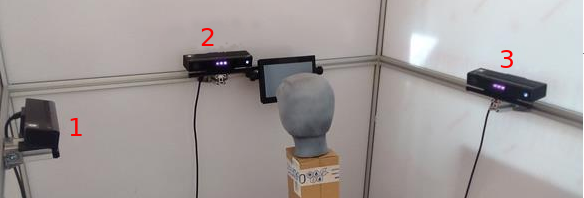
\includegraphics[width=0.9\textwidth]{figures/multicam_placement.png}
	\caption{Rozloženie trojice snímačov Kinect v2 v skenovacej kabíne.}
	\label{fig:multicam:placement}
\end{figure}

Medzi hlavné požiadavky na model sú: hlava musí obsahovať laterálne pohľady (umožniť prekrytie s cefalometrickou snímkou) a orientačné body mäkkého tkaniva.

\begin{figure}[H]
	\centering
	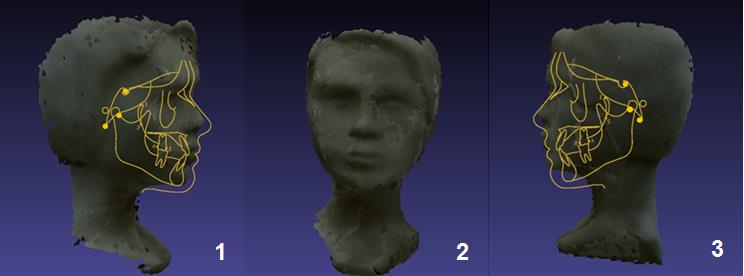
\includegraphics[width=0.9\textwidth]{figures/multicam_placement_scans3.png}
	\caption{Zobrazenie modelov s vyznačenými cefalometrickými parametrami pri použití 3 snímačov. }
	\label{fig:multicam:models}
\end{figure}

Dôležité je aj získanie informácie o šírke krku. Na obrázku \ref{fig:multicam:placement} je zobrazené rozloženie kamier v skenovacej kabíne. Ich jednotlivé 3D modely aj s verifikáciou požiadaviek sa nachádzajú na obr. \ref{fig:multicam:models}. 



\subsection{Sekvenčné snímanie multi-kamerového systému}

Sekvenčný mód predstavuje postupné snímanie. V jednom momente vždy sníma len jedna kamera a ostatné kamery sú vypnuté. Tento režim je pri ToF kamerách často využívaný, pretože tu nevzniká multi-kamerová interferencia. Problémom však je dlhá doba zapínania IR projektora, ktorá pri kamerách Microsoft Kinect v2 dosahuje približne $1s$. Časový odstup medzi dvoma prijatými snímkami je pri $30Hz$ okolo $33ms$.

\subsection{Paralelné snímanie multi-kamerového systému}

V paralelnom režime pracujú všetky kamery v rovnakom čase. Oproti sekvenčnému snímaniu sa inicializácia vykonáva pre každú kameru iba raz. Tým sa radikálne znižuje doba snímania objektu zo všetkých uhlov. Nevýhodou je ale vznik multi-kamerovej interferencie, ktorá dokáže negatívne ovplyvniť výstupné hĺbkové mapy. Časový rozostup medzi jednotlivými snímkami je ovplyvnený samotným spracovaním dát, maximálne však $33ms$ medzi všetkými snímkami. 

\subsection{Porovnanie režimov snímania dynamických objektov}
\label{sec:serial_parallel}
Pre porovnanie týchto režimov bol navrhnutý experiment, pri ktorom sa porovná veľkosť zmeny polohy objektu v závislosti na dĺžke snímania. Pre testovanie bol vyrobený merací prvok, ktorý pozostával z jednosmerného motora, ukazovateľa aktuálnej polohy a statického podstavca slúžiaceho ako uhlomer. Na hriadeli motora bol pripevnený ukazovateľ, ktorý vykonával pohyb po kružnici. Rýchlosť bola nastavená regulovateľným zdrojom tak, aby otočka trvala $5s$. Obvod statického podstavca bol rozdelený na 36 dielov oddelených od seba po $10^\circ$. Kvôli identifikácii polohy podstavec obsahoval zvýraznený nultý bod a šípku informujúcu o smere otáčania ukazovateľa.  

%\begin{figure}[h]
%	\centering
%	\begin{subfigure}[b]{\textwidth}
%		\centering
%		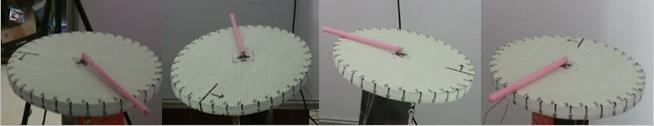
\includegraphics[width=\textwidth]{figures/dynamic_sequence.png}
%		\label{fig:dynamic:sequence}
%	\end{subfigure}
%	\vfill
%	\begin{subfigure}[b]{\textwidth}
%		\centering
%		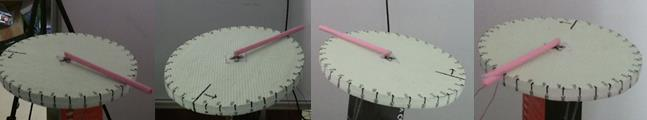
\includegraphics[width=\textwidth]{figures/dynamic_parallel.png}
%		\label{fig:dynamic:parallel}
%	\end{subfigure}
%	\caption{}
%	\label{fig:dynamic:results}
%\end{figure}

Pri sekvenčnom režime boli snímky z kamier získavané postupne od 1. po 4. kameru. Pri paralelnom režime je ťažké identifikovať poradie. Pre porovnanie bolo potrebné získané hĺbkové mapy previesť na mračno bodov a pomocou ICP metódy ich registrovať do jedného modelu (zhodná pozícia nultého bodu). 

\begin{figure}[h]
	\centering
	\begin{subfigure}[b]{0.44\textwidth}
		\centering
		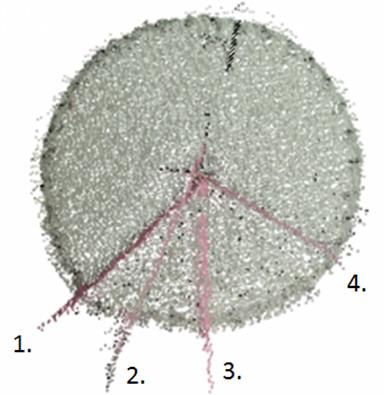
\includegraphics[width=5cm]{figures/dynamic_result_seq.png}
		\caption{}
		\label{fig:dynamic:a}
	\end{subfigure}
	\hskip 8pt 
	\begin{subfigure}[b]{0.44\textwidth}
		\centering
		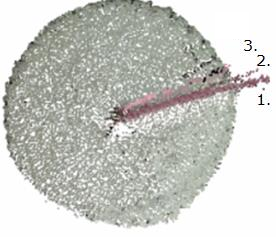
\includegraphics[width=5cm]{figures/dynamic_result_par.png}
		\caption{}
		\label{fig:dynamic:b}
	\end{subfigure}
	\caption{Porovnanie 3D mračien bodov pri rozdielnych režimoch snímania \cite{janisova}: (\textbf{a}) Mračno bodov vytvorené pre sekvenčný režim. (\textbf{b}) Mračno bodov vytvorené pre paralelný režim.}
	\label{fig:dynamic}
\end{figure}


\begin{figure}[H]
	\centering
	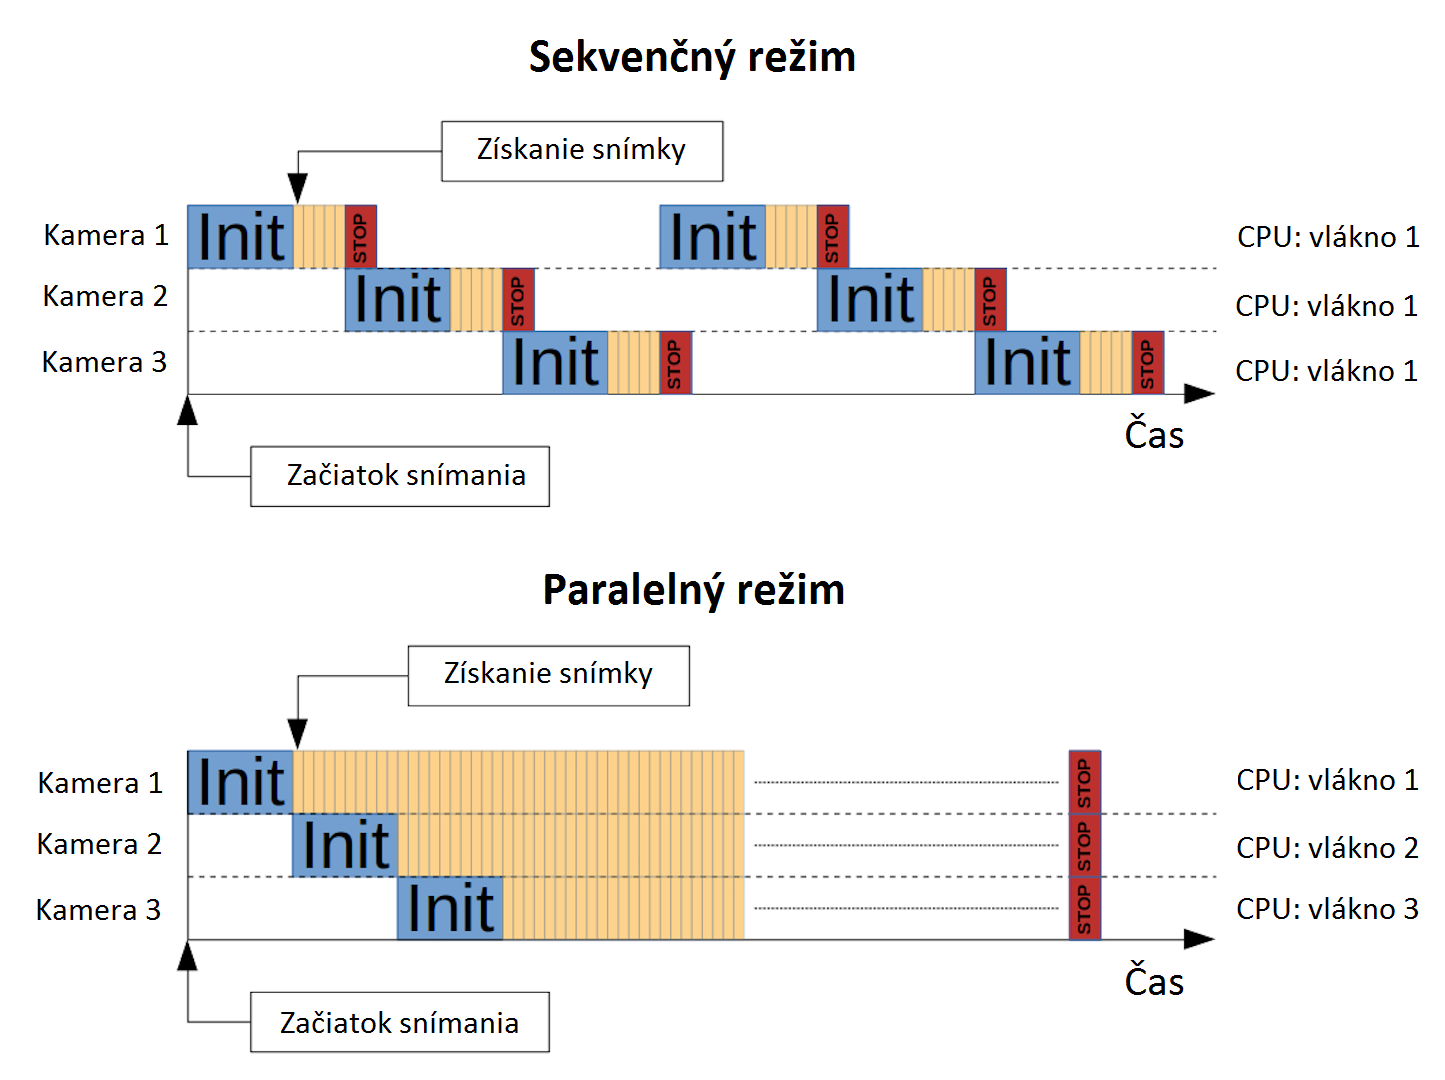
\includegraphics[width=\textwidth]{figures/scanning_mode.png}
	\caption{Grafické porovnanie sekvenčného a paralelného režimu snímania.}
	\label{fig:parallel_sequence}
\end{figure}

Z výsledných modelov je jasne vidieť, že paralelné spracovanie dát má vyšší zmysel pri snímaní dynamických objektov. Pri sekvenčnom režime je rozdiel polohy ukazovateľa výrazný, čo spôsobovalo problémy aj pri ICP registrácií (obr. \ref{fig:dynamic:a}). Naproti tomu je model vytvorený paralelným režimom konzistentnejší, rozdiel polohy ukazovateľa je podstatne menší (obr. \ref{fig:dynamic:b}). Ten by sa dal znížiť hardvérovým synchronizovaným snímaním. Pri kamerách Kinect v2 však táto možnosť chýba a je potrebná. Rozdiel medzi jednotlivými pracovnými režimami sa nachádza na obr. \ref{fig:parallel_sequence}. 

\section{Kalibrácia kamerového systému}
\label{sec:kinect_calib}

Nevyhnutným krokom pri kamerových systémoch je kalibrácia jednotlivých kamier. Pomocou nej sa odstraňuje radiálne a tagenciálne skreslenie, taktiež sa získava matica kamery $P$ (rovnica \ref{eq::pinhole::p}). V tejto kapitole je opísaný postup geometrickej kalibrácie jednotlivých kamier a multi-kamerová kalibrácia. 

\subsection{Geometricka kalibrácia}
Cieľom geometrickej kalibrácie je získanie vnútorných parametrov  kamery spolu s korekčnými parametrami pre odstránenie tangenciálneho a radiálneho skreslenia. Tieto parametre bolo potrebné získať pre RGB aj IR senzory všetkých používaných hĺbkových kamier Kinect v2. 

Pre kalibráciu RGB a IR senzora sa vytvorila séria snímok, ktoré  obsahovali kalibračný vzor snímaný z rôznych uhlov. Ten bol reprezentovaný šachovnicovým motívom o rozmeroch $10\times8$, pričom dĺžka hrany mala veľkosť $36mm$.


%\begin{figure}[h]
%	\centering
%	\begin{subfigure}[b]{0.59\textwidth}
%		\centering
%		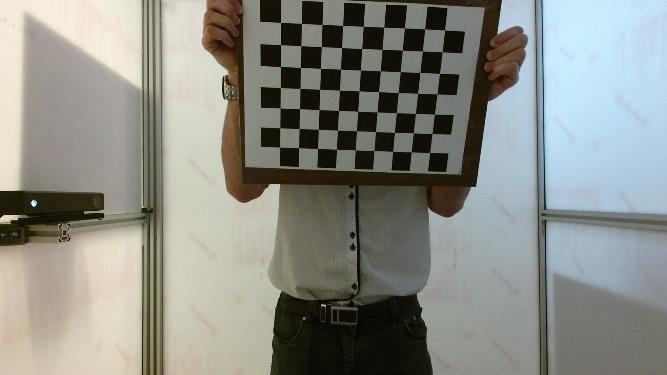
\includegraphics[width=\textwidth]{figures/calibration_rgb.png}
%		\caption{}
%		\label{fig:calib:rgb}
%	\end{subfigure}
%	\hfill
%	\begin{subfigure}[b]{0.4\textwidth}
%		\centering
%		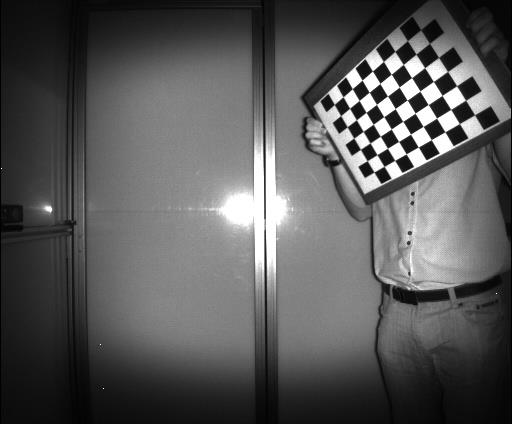
\includegraphics[width=\textwidth]{figures/calibration_ir.png}
%		\caption{}
%		\label{fig:calib:ir}
%	\end{subfigure}
%	\caption{Obrazy z senzora Microsoft Kinect v2: (\textbf{a}) IR obraz bez interferencie. (\textbf{b}) IR obraz s interferenciou. (\textbf{c}) Hĺbková mapa IR obrazu (a). (\textbf{d}) Hĺbková mapa IR obrazu (b). Miesto interferencie je zvýraznené červenou farbou.}
%	\label{fig:calib:single}
%\end{figure}

Pre overenie správnosti kalibrácie IR snímača sa z kalibrovanej a nekalibrovanej hĺbkovej mapy vytvorili mračná bodov. Pri rovnakých podmienkach prostredia bol zosnímaný model hlavy s továrenskými nastaveniami, potom boli použité kalibračné koeficienty získané v predchádzajúcom kroku. Tie boli transformované na trojuholníkovú sieť. Výsledné modely sa porovnávali voči referenčnému modelu. Referenčný model bol vytvorený ručným laserovým skenerom. Ukážky sa nachádzajú na obr. \ref{fig:calib:models}. 

\begin{figure}[H]
	\centering
	\begin{subfigure}[b]{0.32\textwidth}
		\centering
		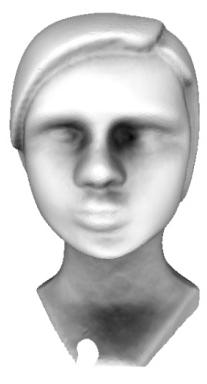
\includegraphics[width=0.59\textwidth]{figures/calibration_models_ref.jpg}
		\caption{}
		\label{fig:calib:model:ref}
	\end{subfigure}
	\hskip 3pt 
	\begin{subfigure}[b]{0.32\textwidth}
		\centering
		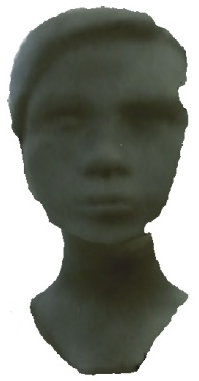
\includegraphics[width=0.57\textwidth]{figures/calibration_models_calib.jpg}
		\caption{}
		\label{fig:calib:model:calib}
	\end{subfigure}
	\hskip 3pt 
	\begin{subfigure}[b]{0.32\textwidth}
		\centering
		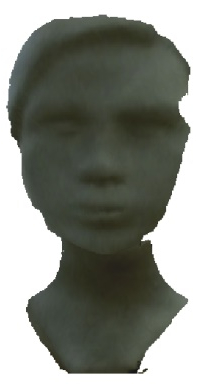
\includegraphics[width=0.57\textwidth]{figures/calibration_models_uncalib.jpg}
		\caption{}
		\label{fig:calib:model:uncalib}
	\end{subfigure}
	\caption{Modely trojuholníkových sietí, použité pre overenie presnosti kalibrácie: (\textbf{a}) Referenčný model objektu vytvorený laserovým snímačom. (\textbf{b}) Model vytvorený z nekalibrovanej kamery Kinect v2. (\textbf{c}) Model vytvorený z kalibrovanej kamery Kinect v2. }
	\label{fig:calib:models}
\end{figure}


Porovnanie priestorovej rekonštrukcie hĺbkových máp bolo robené pomocou Hausdorffovej vzdialenosti.

V nej je detailnejšie zobrazené, aký vplyv má kalibrácia na presnosť rekonštrukcie. Z modelov vzdialenosti (obr. \ref{fig:calib:haus:single}) je vidieť, že nekalibrovaný systém vykazoval vyššiu chybu na okrajoch modelu. To je spôsobené pozitívnym radiálnym skreslením IR senzora, ktorého intenzita je výraznejšia na okrajoch obrazu. Štatistické výsledky pre 10 modelov sa nachádzajú v tabuľke \ref{tab:calib:single}.

\begin{figure}[h]
	\centering
	\begin{subfigure}[b]{0.49\textwidth}
		\centering
		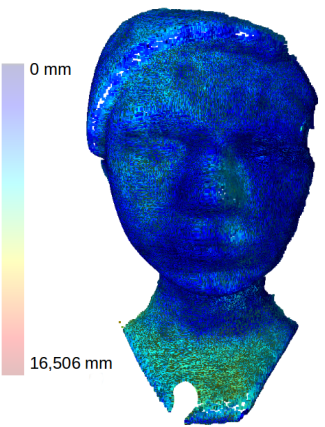
\includegraphics[width=0.57\textwidth]{figures/calibration_hausdorff_single_uncalib.png}
		\caption{}
		\label{fig:calib:haus:single:uncalib}
	\end{subfigure}
	\begin{subfigure}[b]{0.49\textwidth}
		\centering
		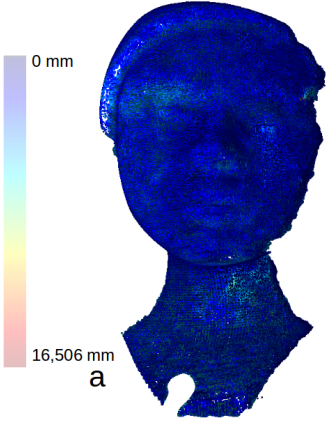
\includegraphics[width=0.57\textwidth]{figures/calibration_hausdorff_single_calib.png}
		\caption{}
		\label{fig:calib:haus:single:calib}
	\end{subfigure}
	\caption{Vizualizácia Hausdorffovej vzdialenosti medzi referenčným modelom (Obr. \ref{fig:calib:model:ref}) a modelom získaným z kamery Kinect v2: (\textbf{a}) Nekalibrovaný systém (výsledok pre model z obr. \ref{fig:calib:model:uncalib}). (\textbf{b}) Kalibrovaný systém (výsledok pre model z obr. \ref{fig:calib:model:calib}).}
	\label{fig:calib:haus:single}
\end{figure}

\begin{table}[H]
	\caption{\label{tab:calib:single} Štatistické porovnanie geometrickej kalibrácie kamier. }
	\centering
	\begin{tabular}{cccc}
		\toprule
		\textbf{Model} & \textbf{Počet meraní [-]} & \textbf{Priemer [mm]} & \textbf{RMS [mm]} \\ 
		\midrule
		\textbf{Nekalibrovaný} & 185187 & 3,0206	& 3,8444 \\
		\textbf{Kalibrovaný} & 296585   & 2,1832   & 2,9506  \\  
		\bottomrule
	\end{tabular}
\end{table}

Týmto krokom sa overil spôsob geometrickej kalibrácie hĺbkových máp. Továrenské nastavenia pre kamery Kinect v2 neposkytujú presné intrinzické parametre a koeficienty skreslenia. V multi-kamerovom systéme, kde sa využíva viacero hĺbkových kamier a vyžaduje sa presnosť rekonštrukcie, je kalibrácia potrebná. 


\subsection{Multi-kamerová kalibrácia}

V tomto procese sa odhadujú vzájomné pozície staticky umiestnených kamier vo svetovej súradnicovej sústave. Ich vzájomnú pozíciu určujú rotačné a translačné parametre (kombinácia afinných transformácií z kapitoly \ref{sec:afine}). Tie je možné získať viacerými spôsobmi. Dôležité je si určiť referenčnú kameru, ktorej matica vonkajších parametrov bude mať tvar identickej afinnej transformácie. Pri multi-kamerovej kalibrácii sa využíva podobný postup ako pri geometrickej kalibrácii. Rozdielom je však, že sa kalibračný vzor sníma súčasne z viacerých kamier. Problém nastáva, ak ich rozloženie neumožňuje súčasné snímanie. Takýto prípad je zachytený na obr. \ref{fig:multicam:placement}.

Riešením je separátne kalibrovanie medzi susednými kamerami (napr. 1-2, 1-3 a 2-4 alebo 3-4). V tomto procese sa vytvorí séria RGB-D párov snímok z jednotlivých dvojíc. Snímky obsahujú rovnaký kalibračný vzor so šachovnicovým motívom. Dôležité je, aby bol vzor staticky umiestnený a nevznikol polohový posun vo dvojici RGB-D mapy. 


\begin{figure}[H]
	\centering
	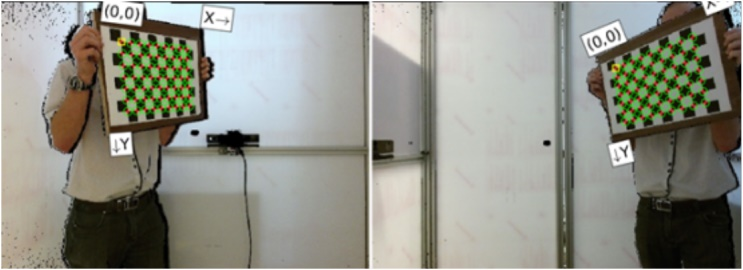
\includegraphics[width=0.7\textwidth]{figures/calibration_multi_rgbd.jpg}
	\caption{Ukážka RGB-D páru použitého pri multi-kamerovej kalibrácii.}
	\label{fig:calib:multi:rgbd}
\end{figure}

Efektívnejším spôsobom je hľadanie vzájomnej pozície kamier cez kľúčové body. V takomto prípade každá staticky umiestnená kamera zosníma kalibračný objekt, z ktorého vygeneruje mračno bodov. V každom mračne sa identifikujú spoločné body, ktoré slúžia na prvotné zarovnanie (\textit{3 point picking alignment}). Následne sa pomocou ICP metódy minimalizuje suma štvorcov euklidovských vzdialeností bodov a vykoná sa jemnejšie zarovnanie. Výhodou statického rozmiestnenia kamier je, že multi-kamerovú kalibráciu je nutné vykonať iba raz. Získaním rotačných a translačných parametrov pre každú kameru získavame zarovnané mračná v spoločnom projektovanom priestore (\ref{tab:calib:multi}). 

\begin{figure}[h]
	\centering
	\begin{subfigure}[b]{0.48\textwidth}
		\centering
		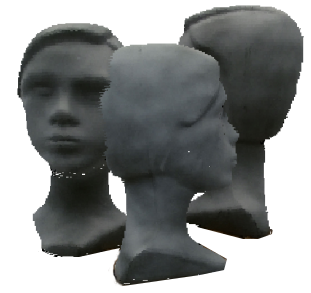
\includegraphics[height=6cm]{figures/calibration_multi_uncalib.png}
		\caption{}
		\label{fig:calib:multi:uncalib}
	\end{subfigure}
	\hfill
	\begin{subfigure}[b]{0.48\textwidth}
		\centering
		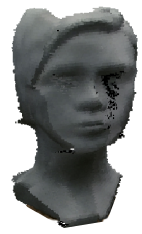
\includegraphics[height=6cm]{figures/calibration_multi_calib.png}
		\caption{}
		\label{fig:calib:haus:calib}
	\end{subfigure}
	\caption{Rekonštruované modely z jednotlivých kamier v spoločnej svetovej súradnicovej sústave: (\textbf{a}) Nekalibrovaná kamerová sústava. (\textbf{b}) Kalibrovaná kamerová sústava.}
	\label{fig:calib:multi}
\end{figure}


\begin{figure}[h]
	\centering
	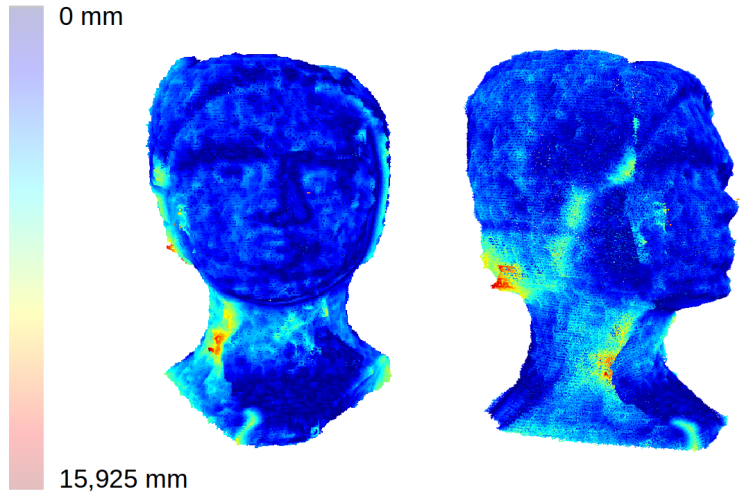
\includegraphics[height=6cm]{figures/calibration_hausdorff_multi.png}
	\caption{Vizualizácia Hausdorffovej vzdialenosti zarovnaných modelov pomocou multi-kamerovej kalibrácie.}
	\label{fig:calib:multi:haus}
\end{figure}

\begin{table}[h]
	\centering
	\caption{\label{tab:calib:multi} Rotačné a translačné parametre pre multi-kamerový systém (topológia systému je na obr. \ref{fig:multicam:placement}). Parameter K predstavuje jednotlivé kamery v tejto sústave. }
	\begin{tabular}{ccccccccccccc}
		\toprule
		\textbf{K} & \textbf{$r_{11}$} & \textbf{$r_{12}$} & \textbf{$r_{13}$} & \textbf{$r_{21}$} & \textbf{$r_{22}$} & \textbf{$r_{23}$} & \textbf{$r_{31}$} & \textbf{$r_{32}$} & \textbf{$r_{33}$} & \textbf{$t_{1}$} & \textbf{$t_{2}$} & \textbf{$t_{3}$} \\ 
		\midrule
		\textbf{1} & 0,2 & -0,1 & 0,99 & -0,74 & 0,15 & 0,98 & 0,1 & -0,09 & -0,99 & 0,08 & 0,04 & 0,62 \\
		\textbf{2} & 1 & 0 & 0 & 0 & 1 & 0 & 0 & 0 & 1 & 0 & 0 & 0 \\ 
		\textbf{3} & 0,09 & 0,16 & -0,98 & 0,56 & -0,14 & 0,98 & 0,15 & -0,07 & 0,99 & 0,13 & 0,11 & 0,5 \\
		\bottomrule
	\end{tabular}
\end{table}

Výsledky Hausdorffovej vzdialenosti medzi referenčným modelom a zarovnaným modelom (trojuholníkové siete) sa nachádzajú v tabuľke \ref{tab:calib:multi:hd}.

\begin{table}[H]
	\caption{\label{tab:calib:multi:hd} Štatistické porovnanie multi-kamerovej kalibrácie kamier. }
	\centering
	\begin{tabular}{cccc}
		\toprule
		\textbf{Model} & \textbf{Počet meraní [-]} & \textbf{Priemer [mm]} & \textbf{RMS [mm]} \\ 
		\midrule
		\textbf{Kalibrovaný} & 1071662   & 2,984   & 3,107  \\  
		\bottomrule
	\end{tabular}
\end{table}

Z výsledkov vyplýva, že priemerná aj RMS chyba je $\sim $ 3mm. Toto zarovnanie je vhodné pre systémy, ktorých rozloženie kamier je statické. Chyba však môže narásť zmenou pracovnej teploty senzora, čím sa ovplyvňuje aj presnosť merania hĺbky (pozri kapitolu \ref{sec:tof}). Z toho dôvodu je potrebné vykonávať ešte jemné zarovnanie mračien pomocou ďalších registračných metód.

\section{Návrh skenovacej metodiky}

Úlohou skenovacej metodiky zloženej z prezentovaných čiastkových algoritmov je vytvoriť konzistentné mračno bodov dynamického objektu z multi-kamerového systému. Toto mračno (model) bude použité pre skríning a automatizovanú diagnostiku OSA v klinickej medicíne. Dynamický objekt je reprezentovaný hlavou pediatrického pacienta. Súčasťou skenovacieho procesu sú algoritmy na podporu automatizovaného merania vybraných kranio-faciálnych parametrov pomocou euklidovskej vzdialenosti. Jadrom a vlastným vedeckým prínosom tejto časti práce je návrh metódy na potláčanie interferenčných artefaktov a vybraných degradačných procesov, na interpoláciu a opravu poškodených častí modelov. Súčasťou metodiky je tiež návrh algoritmu pre segmentáciu hĺbkových máp, ktorý identifikuje a rozdelí jednotlivé časti tváre podľa preddefinovanej klasifikácie.
Z takto segmentovanej hĺbkovej mapy bude možné vytvoriť mračná bodov jednotlivých častí tváre (oči, nos, brada, ústa,...). Takto segmentované oblasti budú v ďalšom výskume použité ako vstupné údaje do procesu automatizovanej diagnostiky. \newline

\noindent Algoritmus môžeme rozdeliť podľa funkcionality na 4 časti: \newline

\begin{compactitem}
	\item Zber a príprava dát v reálnom čase
	\item Spracovanie a filtrácia prijatých dát
	\item Meranie kranio-faciálnych parametrov tváre 
	\item Segmentácia bodov podľa klasifikácie \newline
\end{compactitem}

V prvej časti sa rieši paralelné spracovanie dát zo všetkých pripojených kamier. Vykonáva sa geometrická kalibrácia a základná 2D filtrácia spolu s identifikáciou pohybu tváre. Požiadavka na tento proces je, aby bol vykonávaný v reálnom čase. Ak frekvencia snímania je $30Hz$, časový rozostup medzi snímkami je $33ms$. Preto sú procesy spúšťané paralelne na CPU a GPU. Výstupom z tejto časti je obrazový zásobník, ktorý obsahuje obrazové informácie pediatrického pacienta v pokojovom stave. \newline

\begin{figure}[H]
	\centering
	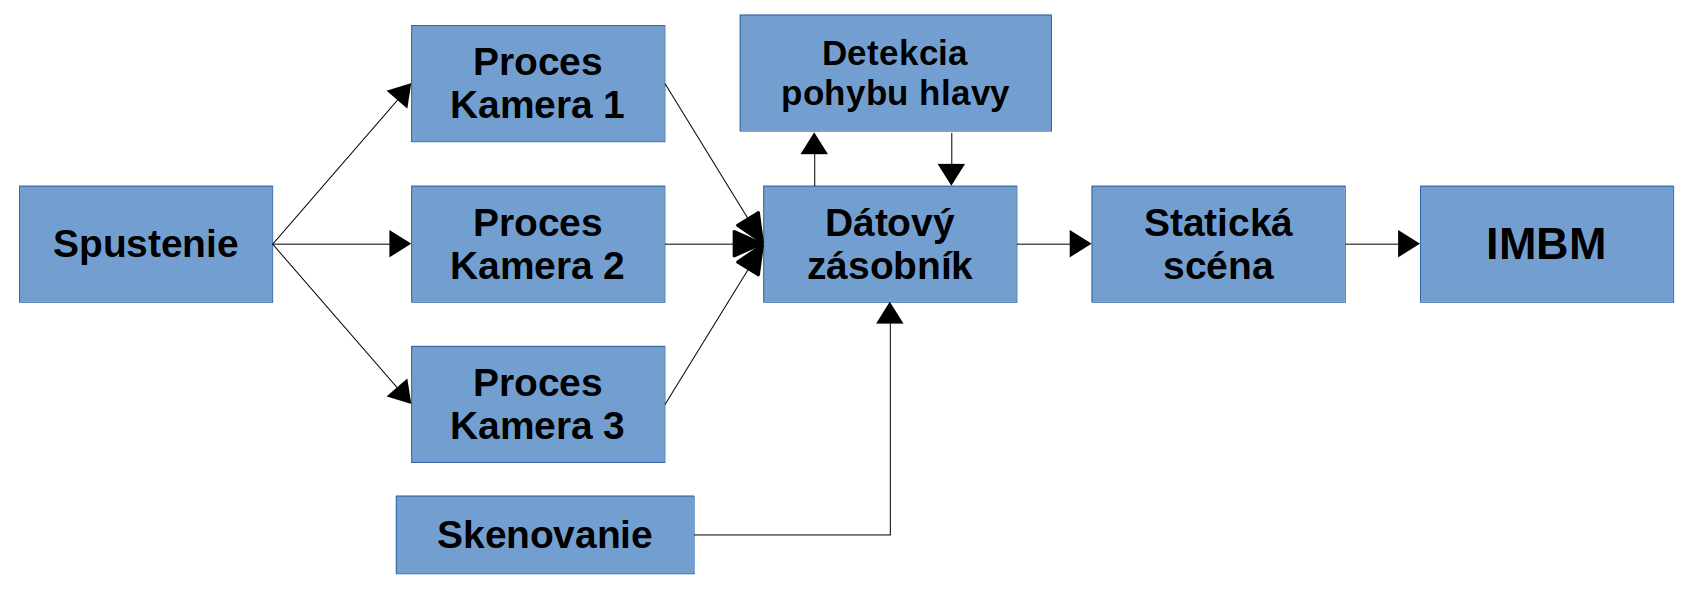
\includegraphics[width=\textwidth]{figures/diagram.png}
	\caption{Diagram algoritmu od inicializácie kamier po IMBM filtráciu.}
	\label{fig:scheme:a}
\end{figure}

V druhej časti sa zo získaných obrazových dát vytvára trojrozmerná reprezentácia snímaného objektu. Prijaté dáta podstupujú filtráciu, ktorou sa zlepšuje kvalita výstupného modelu. Proces využíva štatistické filtre, ktorými sa odstraňujú chybné dáta. Aplikovaním nami navrhnutej metódy IMBM  sa minimalizuje chyba multi-kamerovej kalibrácie. Do priebehu tohto procesu vstupujú aj tretí a štvrtý proces. Tie pracujú s RGB-D obrazmi a hĺbkovými mapami, ktoré sú výstupom IMBM filtrácie (Obr. \ref{fig:scheme:b}). 

\begin{figure}[H]
	\centering
	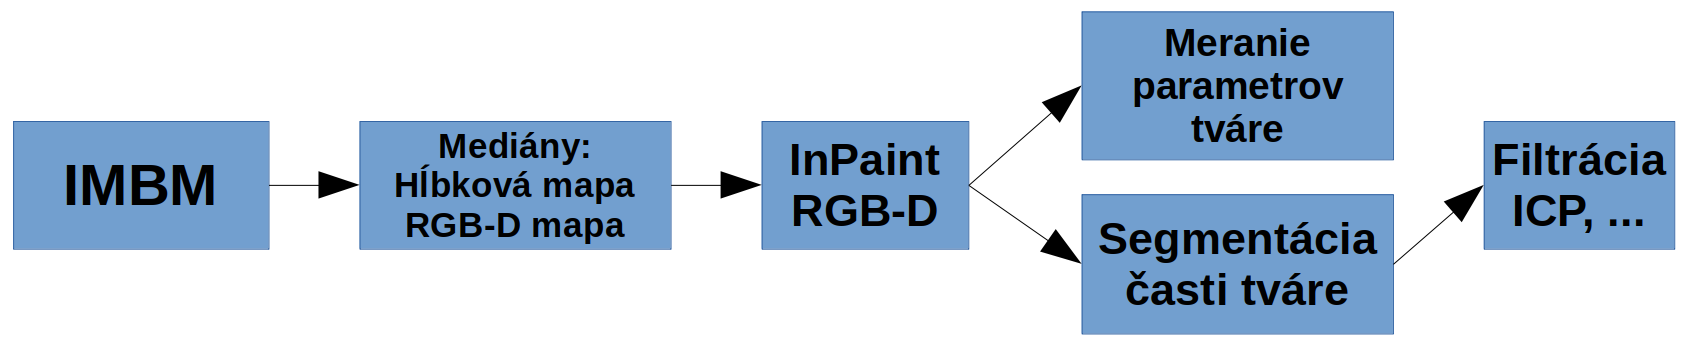
\includegraphics[width=\textwidth]{figures/diagram_post_imbm.png}
	\caption{Diagram spracovania dát po IMBM filtrácii.}
	\label{fig:scheme:b}
\end{figure}

Tretia časť sa zameriava na meranie euklidovských vzdialeností špecifických vybraných parametrov. V RGB-D obraze sa identifikujú kľúčové body, ktoré sú následne prenesené do hĺbkovej mapy. Z týchto bodov sa vypočítajú 3D súradnice a vzdialenosti medzi jednotlivými pármi bodov. Týmto prístupom sa do určitej miery automatizuje vyšetrenie, ktoré je inak vykonávané kontaktným spôsobom. Bezkontaktný prístup je príjemnejší a menej stresujúci pre pediatrických pacientov. Taktiež skracuje dobu vyšetrenia.\newline 

V poslednej fáze sa vykonáva segmentácia výstupných RGB-D obrazov, v ktorých sa hľadajú pixely prislúchajúce jednotlivým častiam ľudskej tváre. Takouto segmentáciou v 2D obraze sa následne dokáže rozdeliť aj ucelené mračno bodov. Výstupom RGB-D segmentácie sú binárne masky, ktoré klasifikujú jednotlivé regióny v hĺbkových mapách. Pri priestorovej rekonštrukcii sa následne konkrétnym bodom nastaví identifikátor, ktorým sa body klasifikujú do tried. Takto je možné rozdeliť jedno zarovnané mračno vytvorené z viacerých hĺbkových máp. 


\subsection{Nástroje použíté pri vývoji algoritmu}

Algoritmus a príslušný softvér bol vyvíjaný v jazyku C++17 na operačnom systéme Linux Mint 18.1. Projekt bol konfigurovaný cez \textit{CMake 3.5}. Využíval pracovné rozhranie \textit{Qt 5.13.9}, v ktorom bolo vyvíjané aj grafické rozhranie projektu. Kamery Kinecvt v2 využívali ovládač \textit{libfreenect2} \cite{blake2015libfreenect2} s podporou \textit{CudaKDE} \cite{lawin2016efficient}. Pre spracovanie 2D obrazu bola použitá knižnica \textit{OpenCV 4}. Pre prácu s 3D dátami sa využívala knižnica \textit{Point Cloud Library 1.9} s vizuálnou podporou knižnice \textit{VTK 6.3}. Identifikácia kľúčových bodov využívala prostriedky \textit{DLib 19.16}. Taktiež sa používali štandardné C++ knižnice a knižnica \textit{Boost 1.63}. Algoritmus využíval procesorové vlákna. Softvér má predpripravené rozhranie pre spoluprácu s kamerami RealSense. 

\subsection{Príprava vstupných dát}
\label{sec:data_prep}
Proces prípravy vstupných dát môžeme rozdeliť na 4 sekvencie.
V prvej sa vykonáva inicializácia kamier a nastavenie konfiguračných parametrov. Medzi základné konfiguračné parametre patria kalibračné koeficienty. Po úspešnej inicializácii sa začína proces snímania. Každé snímanie je vykonávané vo vlastnom CPU vlákne, ktoré je nezávislé od hlavnej slučky programu (Obr. \ref{fig:scheme:c}).

\begin{figure}[H]
	\centering
	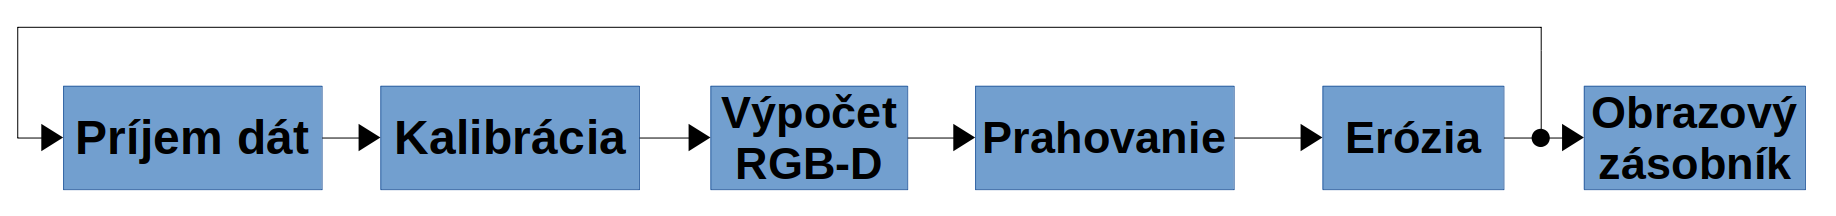
\includegraphics[width=\textwidth]{figures/diagram_cam.png}
	\caption{Sekvencia spracovania prijatých dát z jednotlivých kamier vykonávaná v samostatnom vlákne.}
	\label{fig:scheme:c}
\end{figure}

Každá kamera tak vykonáva úlohy vo vlastnej oddelenej slučke. Samostatne sa tak prijímajú obrazové informácie z jednotlivých kamier. Získava sa 8-bitový RGB obraz, 32-bitový infračervený obraz a taktiež 32-bitová hĺbková mapa. Tieto obrazy sú zbavené skreslenia šošoviek. Mapovaním farebného obrazu na hĺbkovú mapu sa získava RGB-D obraz. Ten popisuje textúru hĺbkovej mapy. Z hĺbkovej mapy je prahovaním odstránené pozadie, pričom hranice prahu sú určené topológiou kamerového systému. Takto vznikne binárna maska objektu, ktorej eróziou zmenšíme plochu na hranách. Pomocou nej je maskovaný RGB-D obraz: 

\begin{description}[leftmargin=*, font=$\bullet$~\normalfont\scshape\color{black}]
	\item[RGB:] 	8-bitový 3-kanálový obraz s rozlíšením $1920 \times 1080$
	\item[IR:]	32-bitový šedo-tonový obraz s rozlíšením $512 \times 424$
	\item[Depth:] Prahovaný 32-bitový šedo-tónový obraz s rozlíšením $512 \times 424$
	\item[RGB-D:] Maskovaný 8-bitový 3-kanálový obraz s rozlíšením $512 \times 424$
\end{description}

V nasledujúcom kroku sa jednotlivé obrazové dáta z kamier ukladajú do dátového zásobníka. Ten sa skladá z obrazových zásobníkov a zásobníkov mračien bodov. Jeho úlohou je spravovať sériu uložených dát, mazať staré a aktualizovať nové. Veľkosť zásobníka je prestaviteľná. Minimálnu hodnotu určuje IMBM filter, ktorý je určený na potlačenie multi-kamerovej interferencie. Jeho spravovanie beží v samostatnom vlákne, čím je znížená časová náročnosť obsluhy jednotlivých dát. Dátový zásobník poskytuje obrazové informácie ďalším procesom. 

Vždy po prijatí nových obrazových dát spustí proces generovania mračna bodov, ktorý beží v samostatnom vlákne. Takto generované mračná slúžia ako 3D nadhľad v grafickom prostredí. Užívateľovi umožňujú vizuálnu kontrolu snímanej scény v reálnom čase (obr. \ref{fig:hmi:a} a \ref{fig:hmi:b}). Body mračna majú štruktúru \textit{XYZRGB}. Kvôli rýchlejšiemu spracovaniu sa organizovaná štruktúra bodov (217088 bodov z hĺbkovej mapy) prevádza na 1D pole, čím je možné odstrániť prebytočné body reprezentované 0 hodnotou pixelu v hĺbkovej mape. Takto sa počet bodov môže redukovať až o $90\%$, čím sa výrazne zníži výpočtová náročnosť. Mračná bodov jednotlivých kamier sa zarovnávajú do spoločného priestoru pomocou extrinzických parametrov získaných pri multi-kamerovej kalibrácii. 

Prácu s grafickým prostredím vykonáva užívateľ, ktorý si zároveň stabilizuje snímaný objekt do požadovanej polohy. Prostredie mu umožňuje vizuálne kontrolovať zmenu polohy a pohyb objektu v reálnom čase. Ak snímaná scéna vyhovuje požiadavkám, užívateľ spustí ďalší proces spracovania dát. V tomto procese sa hľadá séria snímok, kedy poloha objektu vykazuje minimálne zmeny. Táto požiadavka vyplýva z nutnosti použitia IMBM filtrácie. Nasledujúci spôsob detekcie polohy hlavy sa nachádza v ďalšej časti práce. 


\subsection{Identifikácia polohy hlavy}

Z dôvodov, ktoré sú opísané v sekcii \ref{sec:data_prep} je potrebné ukladať sériu snímok do dátového zásobníka. Z dát v zásobníku sa následne generuje mračno bodov, ktoré má čo najvernejšie reprezentovať snímaný objekt. Problém však nastáva, ak je objekt počas doby snímania dynamický. Pohybom môže vzniknúť problém s následným zarovnaním dát do spoločného modelu. Taktiež je veľmi pravdepodobné, že výsledný model nebude geometricky odpovedať skutočným rozmerom. Vplyv pohybových artefaktov je znázornený na \ref{sec:serial_parallel}. Požiadavkou je získať sériu obrazových dát s minimálnou zmenou polohy snímaného objektu.  
Keďže kamery sú staticky umiestnené a zamerané na spoločný centrálny bod, pohyb objektu v hociktorom smere sa prejaví vo všetkých mapách. Tento fakt je rozhodujúci pri návrhu identifikačného systému. Z toho logicky vyplýva, že stačí analyzovať pohyb objektu len z dát jednej kamery. Identifikovanie kľúčových bodov, ktoré budú zhodné pre každú snímku v obrazovom zásobníku pomôže vypočítať pohyb a rozptyl polohy. \newline

Ak je pixel $P$ reprezentovaný konkrétnym stĺpcom $r_{i}$ a riadkom $c_{i}$, tak bod záujmu $P_{i}$ predstavuje jedinečnú pozíciu v obraze. Index $i$ predstavuje konkrétny kľúčový bod detektora a $N$ snímku v zásobníku. Bodu $P_{i}$ prislúcha informácia o farbe $R_{i};G_{i};B_{i}$ (získanej z RGB-D obrazu) a o hĺbke $d_{i}$ (získanej z hĺbkovej mapy).

\begin{equation}
\label{eq:pixels:a}
\begin{aligned}
P_{i}=P\left(r_{i};c_{i}\right)
\end{aligned}
\end{equation}
\begin{equation}
\label{eq:pixels:b}
\begin{aligned}
P_{i;N}=P\left(r_{i;N};c_{i;N}\right)
\end{aligned}
\end{equation}
\begin{equation}
\label{eq:pixels:c}
\begin{aligned}
P_{i}=R_{i};G_{i};B_{i};d_{i}
\end{aligned}
\end{equation}

\noindent Rozptyl polohy kľúčového bodu $P_d$ sa vypočíta ako absolútna hodnota rozdielu maximálnej a minimálnej pozície pixelu v danom smere. 

\begin{equation}
\label{eq:pixels:d}
\begin{aligned}
P_d\left(x\right)=\left|  max\lbrace c_{i;N} \rbrace -min\lbrace c_{i;N} \rbrace \right| 
\end{aligned}
\end{equation}
\begin{equation}
\label{eq:pixels:e}
\begin{aligned}
P_d\left(y\right)=\left|  max\lbrace r_{i;N} \rbrace -min\lbrace r_{i;N} \rbrace \right| 
\end{aligned}
\end{equation}
\begin{equation}
\label{eq:pixels:f}
\begin{aligned}
P_d\left(z\right)=\left|  max\lbrace d_{i;N} \rbrace -min\lbrace d_{i;N} \rbrace \right| 
\end{aligned}
\end{equation}

Úlohou algoritmu je identifikovať, kedy rozptyl bodov $P_d$ v každom smere neprekročí stanovenú hranicu. Identifikácia sa začína interakciou užívateľa systému (doktor) s grafickým prostredím programu. Snímaný objekt musí byť v pokojovom stave a nastavenej pozícii. Príklad RGB-D obrazov dynamického objektu, ktoré môžu byť použité na detekciu kľúčových bodov, sa nachádza na obr. \ref{fig:dlib:views}. 

\begin{figure}[H]
	\centering
	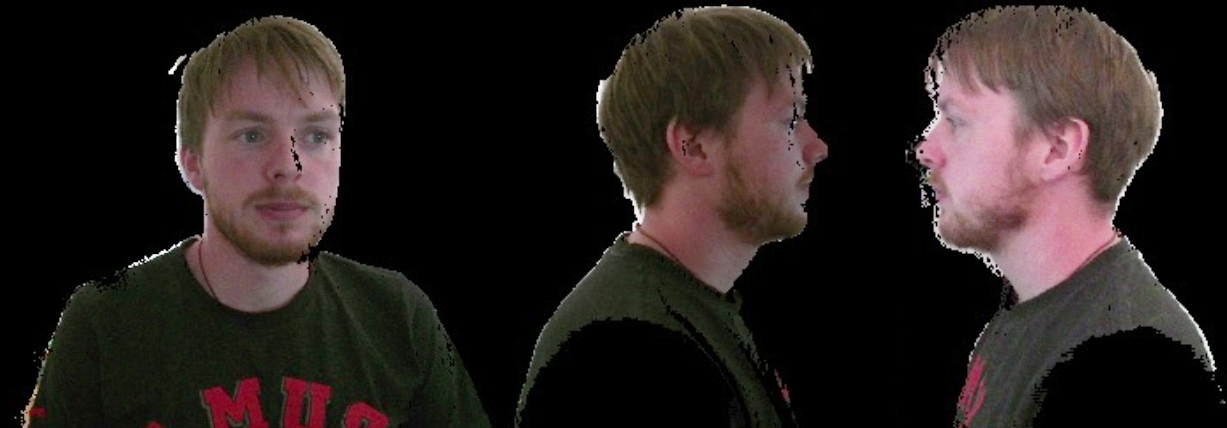
\includegraphics[width=0.9\textwidth]{figures/rgbd_views.png}
	\caption{Prahované RGB-D snímky vytvorené multi-kamerovým systémom zachytávajúce dynamický objekt v rovnakom čase.}
	\label{fig:dlib:views}
\end{figure}

Pohybová aktivita je znížená vplyvom podporného vizualizačného systému (tablet premietajúci zaujímavý obsah), ktorého úlohou je udržať pohľad objektu koncentrovaný na jedno miesto.

Ideálny je frontálny pohľad, pretože tvár obsahuje veľa statických a jedinečných prvkov. V súčasnosti existuje niekoľko desiatok metód, ktoré sú určené na detekciu tváre a jej orientačných bodov. Ich úlohou je čo najpresnejšie identifikovať spomínané body. V tejto práci sa používa detektor DLib, ktorý pracuje na princípe súboru regresívnych stromov \cite{king2009dlib}. Výhodou použitia DLib detektora oproti SURF a SIFT metódam je, že dokážu ľahko identifikovať aj mimiku tváre. Takýmto spôsobom sa umožňuje detekcia pohybu hlavy pri rôznych polohách a tvárových výrazoch. 
Základný detektor identifikuje 68 bodov tváre, pričom vie ohraničiť tvár, oči, nos a ústa. Ukážka aplikácie detektora na RGB-D obraze sa nachádza na obrázku \ref{fig:dlib:points}.

\begin{figure}[H]
	\centering
	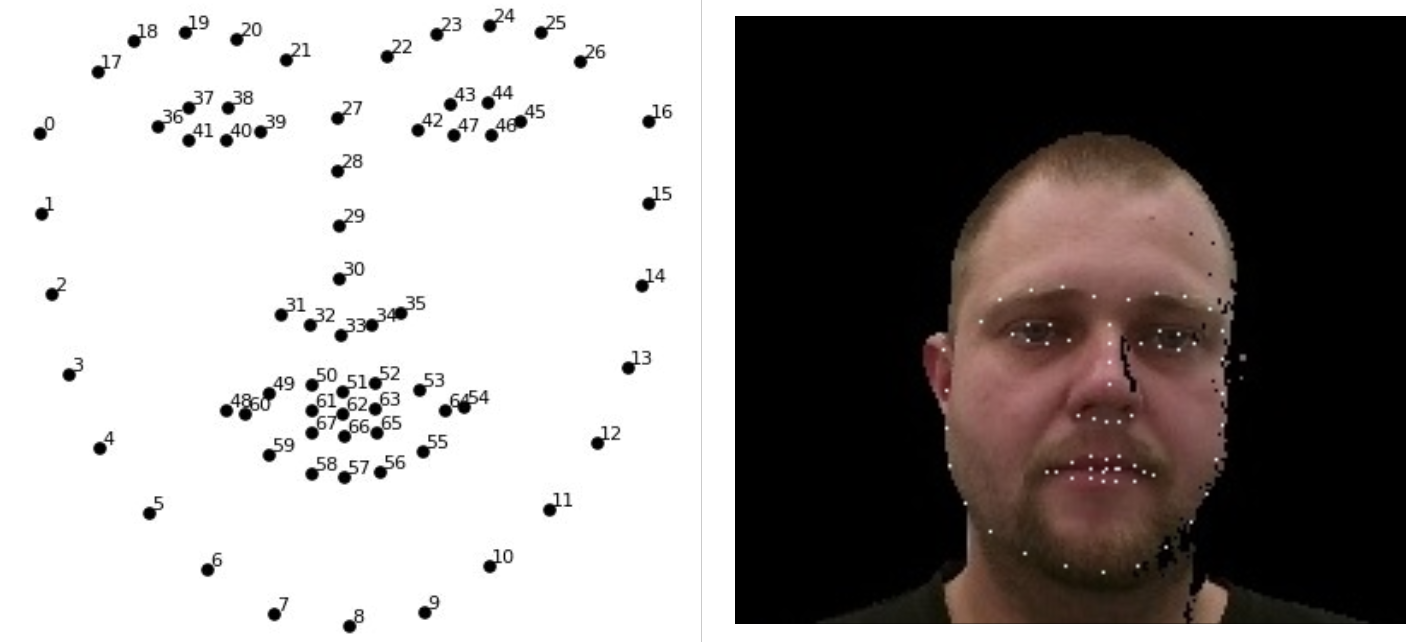
\includegraphics[width=0.90\textwidth]{figures/face_landmarks.png}
	\caption{\textbf{Vľavo:} Označenie 68 základných kľúčových bodov \textit{ DLib Face Landmark} detektora \cite{king2009dlib}.  \textbf{Vpravo:} Aplikácia na RGB-D obraze získanej z kamery Kinect v2.}
	\label{fig:dlib:points}
\end{figure}
 
Problém nastáva pri chýbajúcich dátach v RGB-D obraze, ktoré vznikajú pri mapovaní RGB obrazu na poškodenú hĺbkovú mapu. Kvôli spracovaniu v reálnom čase je detekcia vykonávaná ešte pred filtráciou a opravou RGB-D obrazu. Preto sa k detekcii používajú ešte nefiltrované dáta. Na nich môže dochádzať k nesprávnej detekcii bodov. Problematické sú aj body 0 až 16, pretože v závislosti na fenotype tváre sa ich umiestnenie môže vyskytnúť mimo objektu. 

Redukovanie počtu detekovaných kľúčových bodov na minimálny počet zabezpečí zníženie stavu, kedy bude mať bod $P_i$ hodnotu $d_i=0$. K nasledujúcej detekcii bol použitý detektor identifikujúci 5 kľúčových bodov. 
 
\begin{figure}[H]
	\centering
	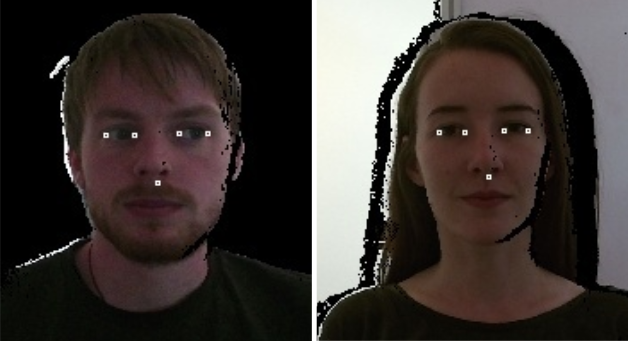
\includegraphics[width=0.70\textwidth]{figures/rgbd_points.png}
	\caption{DLib detektor identifikujúci 5 kľúčových bodov tváre na RGB-D obraze.}
	\label{fig:dlib:rbbd5}
\end{figure}

\noindent Z RGB-D obrazu (obr. \ref{fig:dlib:rbbd5}) sa následne pozície kľúčových bodov $r_i, c_i$ prenesú do hĺbkovej mapy. Získajú sa hĺbkové informácie $d_i$ a vypočítajú sa hodnoty $P_d$. 

\begin{figure}[H]
	\centering
	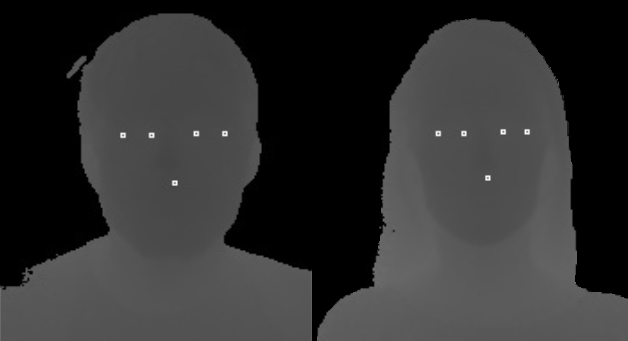
\includegraphics[width=0.72\textwidth]{figures/depth_points.png}
	\caption{Prenesenie identifikovaných kľúčových bodov z RGB-D obrazu (Obr. \ref{fig:dlib:rbbd5}) do hĺbkovej mapy.}
	\label{fig:dlib:depth5}
\end{figure}

Pre porovnanie 5 a 68 bodového detektora sa štatisticky analyzovalo, koľko detekovaných bodov malo nulovú hodnotu hĺbky $d_i=0$. Zároveň sa zisťoval súčet hĺbkových máp, v ktorých mali detekované body 0 hodnotu $F(d_i=0)$. V tabuľke \ref{tab:dlib:compare} sú zobrazené výsledky z 87 testovacích snímok.  

\begin{table}[h]
	\caption{\label{tab:dlib:compare} Štatistické porovnanie 68 bodového a 5 bodového detektora na 87 hĺbkových mapách.}
	\centering
	\begin{tabular}{lccccc}
		\toprule
		\textbf{Model} & \textbf{Počet bodov} & \textbf{$d_i=0$} & \textbf{$F(d_i=0)$} & \textbf{$d_i=0 [\%]$ } & \textbf{$F(d_i=0) [\%]$} \\ 
		\midrule
		\textbf{5 bodov} 	& 415 	& 2		& 2		& 0,48	& 2,298 \\
		\textbf{68 bodov} 	& 5644	& 41 	& 23	& 0,72	& 26,437 \\
		\bottomrule
	\end{tabular}
\end{table}

Oba detektory mali veľmi nízku hodnotu prípadov, kedy identifikovanému bodu $P_i$ chýbala hĺbková informácia. Avšak pri 68 bodovom detektore približne každý štvrtý snímok obsahoval takýto bod. 


Pre porovnanie stability detekcie kľučových bodov sme vykonali meranie euklidovských vzdialeností $d_e$ medzi jednotlivými bodmi. Zisťovaná bola šírka ľavého a pravého oka, vonkajší a vnútorný rozostup očí. Meranie bolo vykonané na datasete, ktorý obsahoval 135 párov snímok (RGB-D, hĺbková mapa) pre oba detektory.

\begin{equation}
\label{eq:euclidean}
\begin{aligned}
d_{e}\left(P_i,P_j\right)= \sqrt{\left(P_i(x) - P_j(x)\right)^2 + \left(P_i(y) - P_j(y)\right)^2 + \left(P_i(z) - P_j(z)\right)^2} 
\end{aligned}
\end{equation}

Z výsledkov sa vypočítal medián, priemerná hodnota a rozdiel medzi maximálnou a minimálnou nameranou hodnotou. Údaje pre jednotlivé detektory sa nachádzajú v tabuľkách \ref{tab:dlib:5points} a \ref{tab:dlib:68points}.
 
\begin{table}[h]
	\caption{\label{tab:dlib:5points} Meranie vybraných faciálnych rozmerov pomocou 5 bodového detektora.}
	\centering
	\begin{tabular}{lccc}
		\toprule
		\textbf{Meranie} & \textbf{Medián [mm]} & \textbf{Priemer [mm]} & \textbf{Rozdiel (Max-Min) [mm]} \\ 
		\midrule
		\textbf{Šírka ľavého oka} 	& 28,38 & 28,41	& 5,03 \\
		\textbf{Šírka pravého oka} 	& 26,21	& 26,17 & 4,39 \\
		\textbf{Vnút. rozostup očí} 	& 38,43	& 38,22 & 2,32 \\
		\textbf{Vonk. rozostup očí} 	& 90,06	& 89,89 & 3,22 \\
		\bottomrule
	\end{tabular}
\end{table}

\begin{table}[h]
	\caption{\label{tab:dlib:68points} Meranie vybraných faciálnych rozmerov pomocou 68 bodového detektora.}
	\centering
	\begin{tabular}{lccc}
		\toprule
		\textbf{Meranie} & \textbf{Medián [mm]} & \textbf{Priemer [mm]} & \textbf{Rozdiel  (Max-Min) [mm]} \\ 
		\midrule
		\textbf{Šírka ľavého oka} 	& 28,46 & 28,52	& 5,40 \\
		\textbf{Šírka pravého oka} 	& 27,13	& 27,22 & 4,81 \\
		\textbf{Vnút. rozostup očí} 	& 37,13	& 37,00 & 3,16 \\
		\textbf{Vonk. rozostup očí} 	& 85,99	& 89,70 & 4,16 \\
		\bottomrule
	\end{tabular}
\end{table}

V nich môžeme vidieť, že výsledky sú podobné. Dôležitým parametrom je rozdiel medzi maximálnou a minimálnou nameranou hodnotou. Ten hovorí o tom, ako stabilná je detekcia kľúčových bodov pri rôznych polohách tváre. Rozptyl detekovaných bodov je priamo úmerný veľkosti rozdielu medzi maximálnou a minimálnou hodnotou.

\begin{table}[H]
	\caption{\label{tab:dlib:resulrs} Rozdiel výsledkov medzi 68 a 5 bodovým detektorom.}
	\centering
	\begin{tabular}{lccc}
		\toprule
		\textbf{Meranie} & \textbf{Medián [mm]} & \textbf{Priemer [mm]} & \textbf{Rozdiel (Max-Min) [mm]} \\ 
		\midrule
		\textbf{Šírka ľavého oka} 	& -0,08 & -0,11	& -0,38 \\
		\textbf{Šírka pravého oka} 	& -0,93	& -1,05 & -0,42 \\
		\textbf{Vnút. rozostup očí} 	& 1,30	& 1,21 & -0,83 \\
		\textbf{Vonk. rozostup očí} 	& 0,51	& 0,19 & -0,93 \\
		\bottomrule
	\end{tabular}
\end{table}

Pre lepšie porovnanie sme odčítali výsledky merania 5 bodového detektora od 68 bodového detektora. Z výsledkov vyplýva, že rozdiel medzi presnosťou jednotlivých detektorov je minimálny. Maximálna hodnota rozdielu je $1.3mm$ pri meraní vnútorného rozostupu očí. Z tohto experimentu vyplýva, že oba detektory sú vhodné pre meranie pohybu tváre. Každý z nich lokalizuje body pod $33ms$, čo je podmienka pri práci v reálnom čase. 68 bodový detektor má potenciálne využitie pri meraní tváre v rôznych mimikách (úsmev, ...). Tieto mimiky majú potenciál pri diagnostike OSA.
  

\subsection{Filtrácia a registrácia mračna bodov}
\label{sec:filtration}
V predchádzajúcom kroku sa zabezpečilo získanie série snímok, ktoré zachytávali objekt v statickej polohe (alebo pri minimálnych pohyboch). Veľkosť série snímok určuje IMBM filter, ktorého detailný opis a optimálne nastavenia sa nachádzajú v kapitole \ref{kap:interference}. Podstatnými dátami sú hĺbkové mapy a RGB-D obrazy jednotlivých pohľadov. Tieto dáta už podstúpili jednoduchú filtráciu akou bola erózia a prahovanie (pozri \ref{fig:dlib:rbbd5} a \ref{fig:dlib:depth5}). 

V ďalšom kroku sa vykonáva IMBM filtrácia, ktorej úlohou je identifikovať a odstrániť multi-kamerovú interferenciu. Multi-kamerová interferencia je v tomto prípade dôsledok využitia paralelnej spolupráce viacerých ToF kamier. Spôsobuje zašumenie hĺbkovej mapy a vznik odľahlých pixelov. IMBM filter dokáže identifikovať interferujúce miesta a odstrániť chybné pixely. 

Filter pracuje s hĺbkovými mapami, výstupom z filtra je taktiež hĺbková mapa. Pre lepšiu vizualizáciu funkčnosti jednotlivých krokov IMBM sú hĺbkové mapy prevedené do mračien bodov.  

\begin{figure}[h]
	\centering
	\begin{subfigure}[b]{0.32\textwidth}
		\centering
		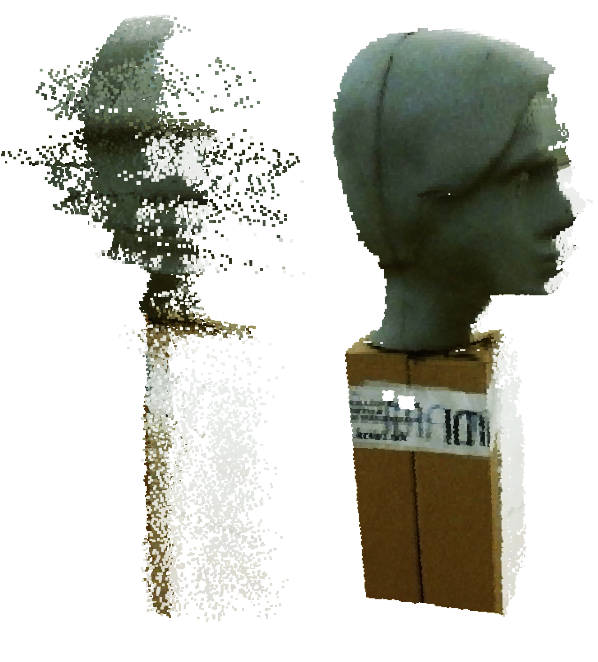
\includegraphics[height=4.4cm]{figures/prepared_models_a.png}
		\caption{}
		\label{fig:imbm:result:a}
	\end{subfigure}
	\hfill
	\begin{subfigure}[b]{0.32\textwidth}
		\centering
		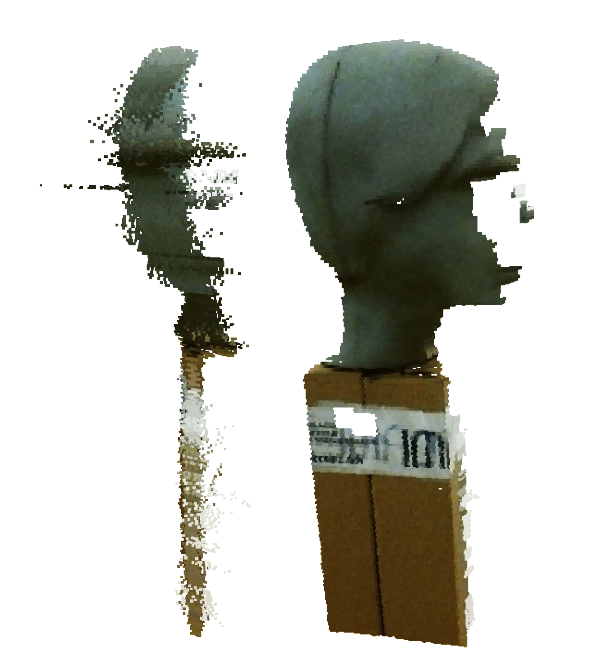
\includegraphics[height=4.4cm]{figures/prepared_models_b.png}
		\caption{}
		\label{fig:imbm:result:b}
	\end{subfigure}
	\hfill
	\begin{subfigure}[b]{0.32\textwidth}
		\centering
		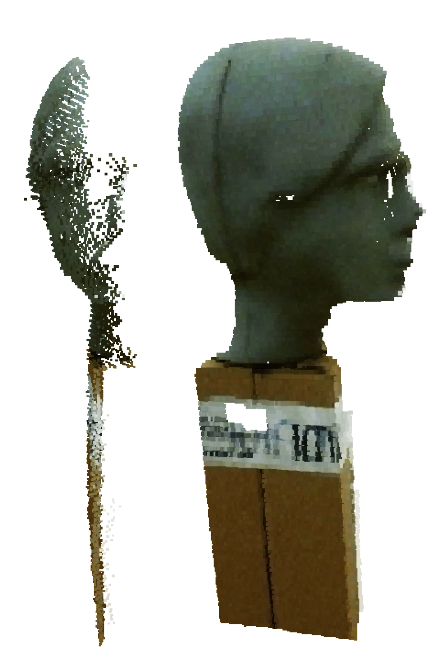
\includegraphics[height=4.4cm]{figures/prepared_models_c.png}
		\caption{}
		\label{fig:imbm:result:c}
	\end{subfigure}
	\caption{IMBM filtrácia: (\textbf{a}) Ukážka vplyvu interferencie. (\textbf{b}) Extrakcia interferovaných miest. (\textbf{c}) Filtrované dáta s interpolovaním chybných miest.}
	\label{fig:imbm:result}
\end{figure}

Ukážka vplyvu interferencie na mračno bodov sa nachádza na obr. \ref{fig:imbm:result:a}. To je vytvorené zo série hĺbkových máp jednej kamery. Model obsahuje veľké množstvo chybných pixelov, ktoré sú rozptýlené okolo povrchu modelu. Navyše sa interferencia prejavuje v oblasti komplexnej geometrickej štruktúry. 
Na obr. \ref{fig:imbm:result:b} sa nachádza mračno bodov po odstránení poškodených regiónov vytvorené z jednej hĺbkovej mapy. V porovnaní s prvým modelom je vidieť, že oblasť interferencie je značná. Tento model stále obsahuje šum a interferenčné miesta, ktoré neboli identifikované IMBM filtrom.  
Výsledné mračno bodov (obr. \ref{fig:imbm:result:c}) je vytvorené zo stredných hodnôt jednotlivých filtrovaných mračien bodov. Tento model má podstatne znížený šum a počet lietajúcich pixelov bez straty interferovaných regiónov. Filtráciou však môžu v modeli vzniknúť diery. Ak sú malé a nenachádzajú sa v komplexných oblastiach, IMBM dokáže tieto hodnoty interpolovať. 

Výstupný RGB-D obraz z IMBM je priemerom vstupných RGB-D obrazov. Pomocou tohto obrazu sa nanáša textúra na mračno bodov. Na obr. \ref{fig:dlib:rbbd5} je vidieť, že vstupné obrazy obsahujú prázdne miesta (0 hodnoty pixelov) aj v oblastiach, kde hĺbka nie je nulová.
Tieto miesta sú do určitej miery odstránené vo výstupnom RGB-D obraze.


\begin{figure}[h]
	\centering
	\begin{subfigure}[b]{0.48\textwidth}
		\centering
		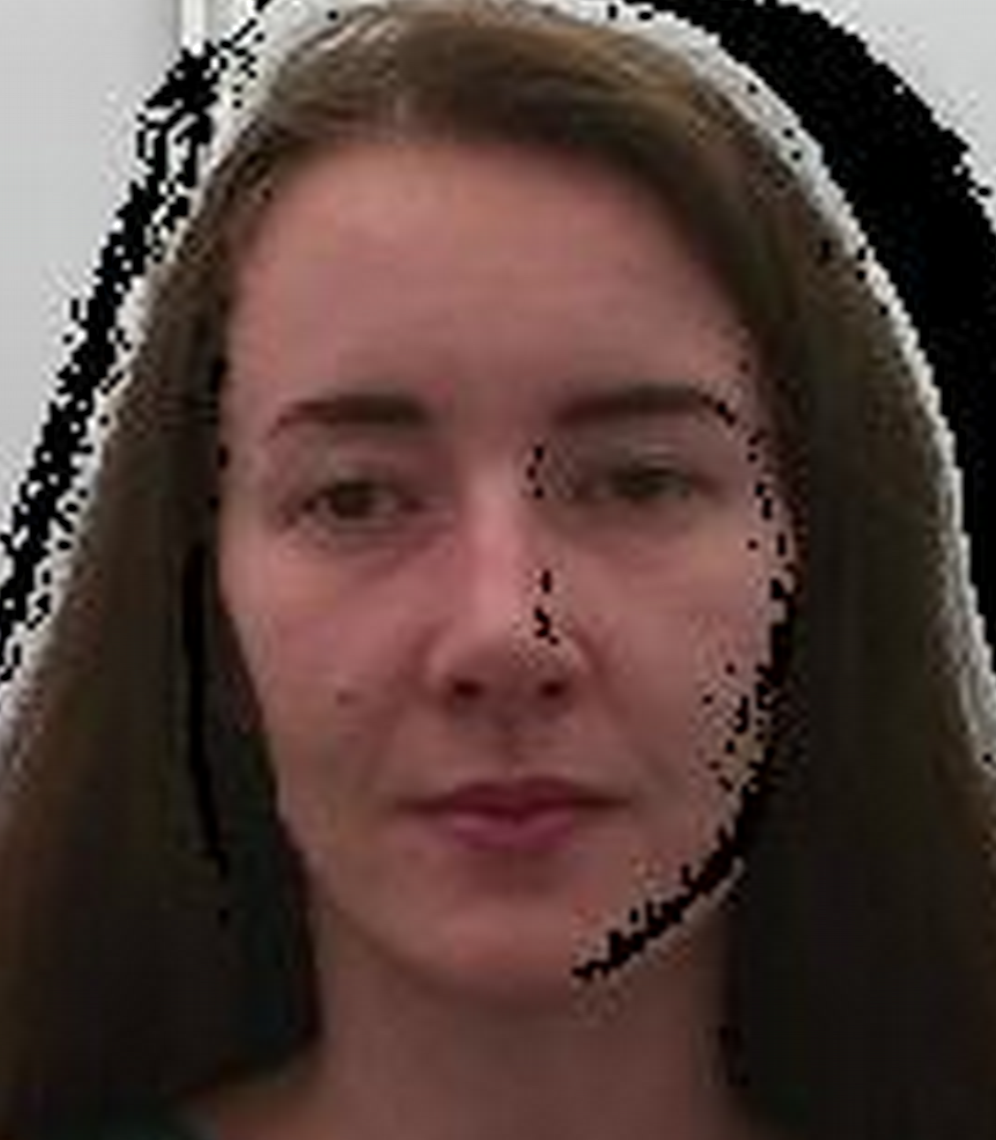
\includegraphics[height=4.4cm]{figures/inpaint_a.png}
		\caption{}
		\label{fig:inpaint:a}
	\end{subfigure}
	\hskip 0in
	\begin{subfigure}[b]{0.48\textwidth}
		\centering
		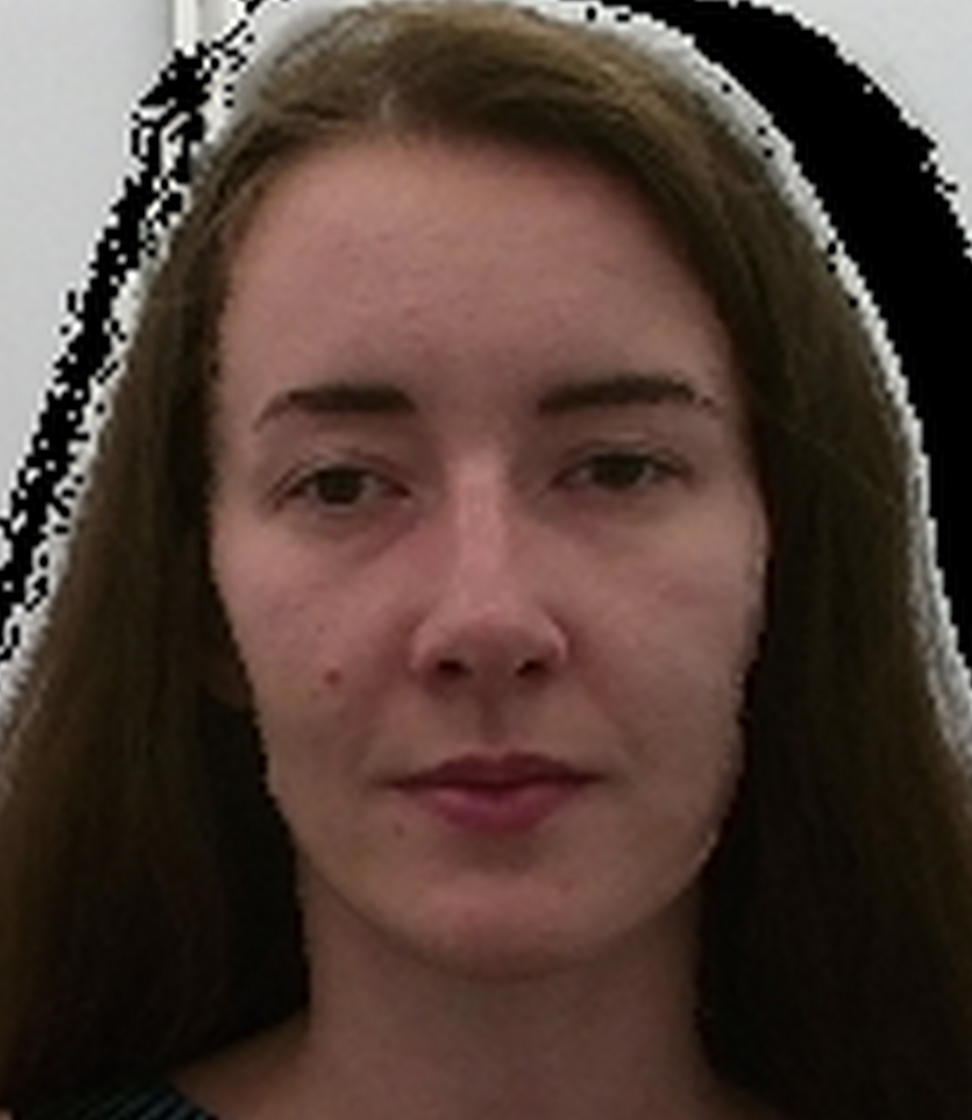
\includegraphics[height=4.4cm]{figures/inpaint_b.png}
		\caption{}
		\label{fig:inpaint:b}
	\end{subfigure}
	\caption{Oprava RGB-D obrazu pomocou metódy Telea : (\textbf{a})Výstupný  medián RGB-D mapy s poškodenými ROI. (\textbf{b}) Oprava farebnej informácie na miestach, kde sa v hĺbkovej mape nachádza objekt.}
	\label{fig:inpaint}
\end{figure}

K úplnému odstráneniu poškodených miest používame Teleovú metódu \cite{telea2004image}. K aplikácii použijeme hĺbkovú mapu a RGB-D obraz z IMBM filtra. Opravujeme len pixely, ktoré majú súčet R,G a B vrstiev rovný 0 a hĺbková informácia $d$ je rôzna od 0. Výstupom je RGB-D obraz, ktorý je zbavený poškodených miest (Obr. \ref{fig:inpaint}).

Po tomto kroku máme pripravené mediány hĺbkových máp, ktoré sú použité pri meraní kranio-faciálnych parametrov tváre a pri segmentácii hĺbkovej mapy. Tieto spracovania sú opísané v samostatných kapitolách. Z týchto dát následne vytvárame mračná bodov. Pomocou nasledujúcich rovníc prebieha rekonštrukcia snímaného priestoru. 

\begin{equation}
\label{eq:project:x}
\begin{aligned}
x=\dfrac{P_{i}(c_{i})+0.5-c_{x}}{f_{x}}P_{i}(d_{i})
\end{aligned}
\end{equation}
\begin{equation}
\label{eq:project:y}
\begin{aligned}
y=\dfrac{P_{i}(r_{i})+0.5-c_{y}}{f_{y}}P_{i}(d_{i})
\end{aligned}
\end{equation}
\begin{equation}
\label{eq:project:z}
\begin{aligned}
z=P_{i}(d_{i})
\end{aligned}
\end{equation}

Intrinzické parametre $c_x, c_y, f_x, f_y$ sú unikátne pre každú kameru a sú výstupom geometrickej kalibrácie kamier. Parametre $P_i(c_i),P_i(r_i)$ sa odkazujú na rovnice (\ref{eq:pixels:a}) až (\ref{eq:pixels:c}). Pomocou rotačných a translačných parametrov, ktoré boli získane pri viac-kamerovej kalibrácii, zarovnávame mračná bodov z jednotlivých kamier do spoločnej súradnicovej sústavy. Tieto mračná sú filtrované pomocou \textit{Radius Outlier Removal} filtra (ROR). Bližší opis tohto filtra sa nachádza v kapitole \ref{sec:ror}. 


\begin{figure}[h]
	\centering
	\begin{subfigure}[b]{0.32\textwidth}
		\centering
		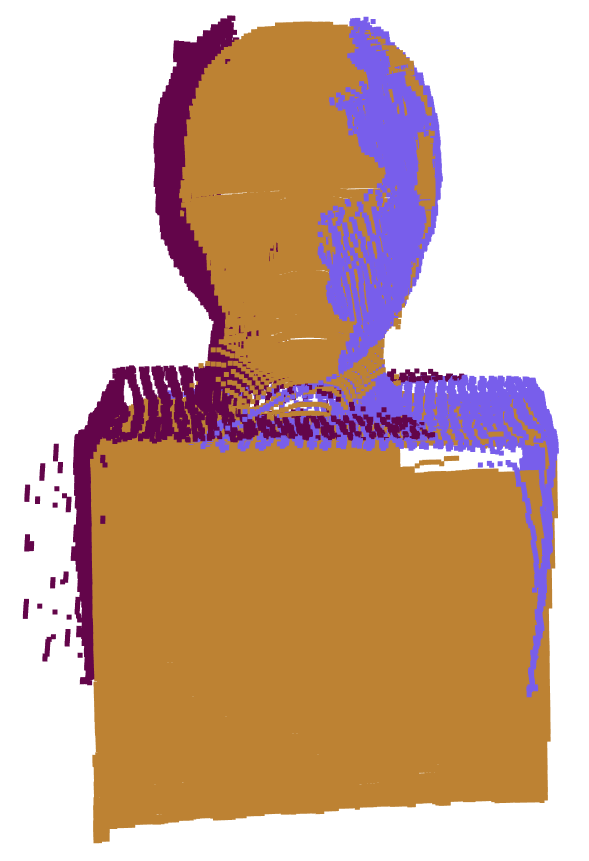
\includegraphics[height=4.9cm]{figures/model_colors.png}
		\caption{}
		\label{fig:ror:a}
	\end{subfigure}
	\hfill
	\begin{subfigure}[b]{0.32\textwidth}
		\centering
		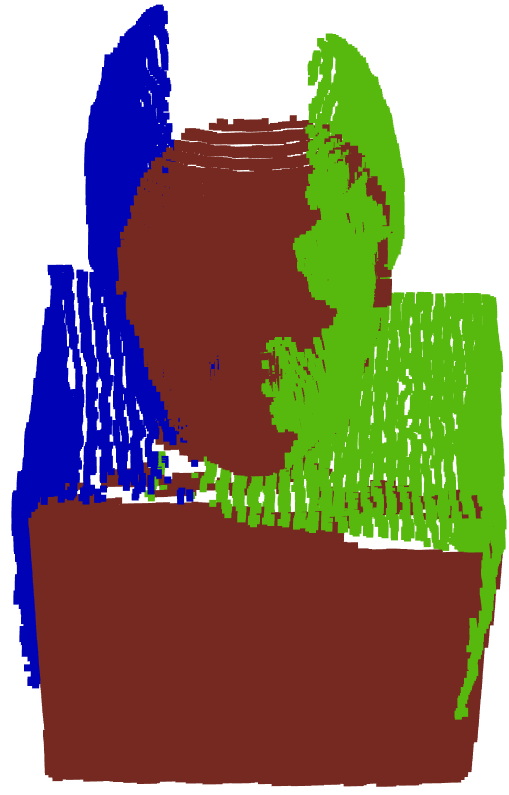
\includegraphics[height=4.9cm]{figures/ror_preserv.png}
		\caption{}
		\label{fig:ror:b}
	\end{subfigure}
	\hfill
	\begin{subfigure}[b]{0.32\textwidth}
		\centering
		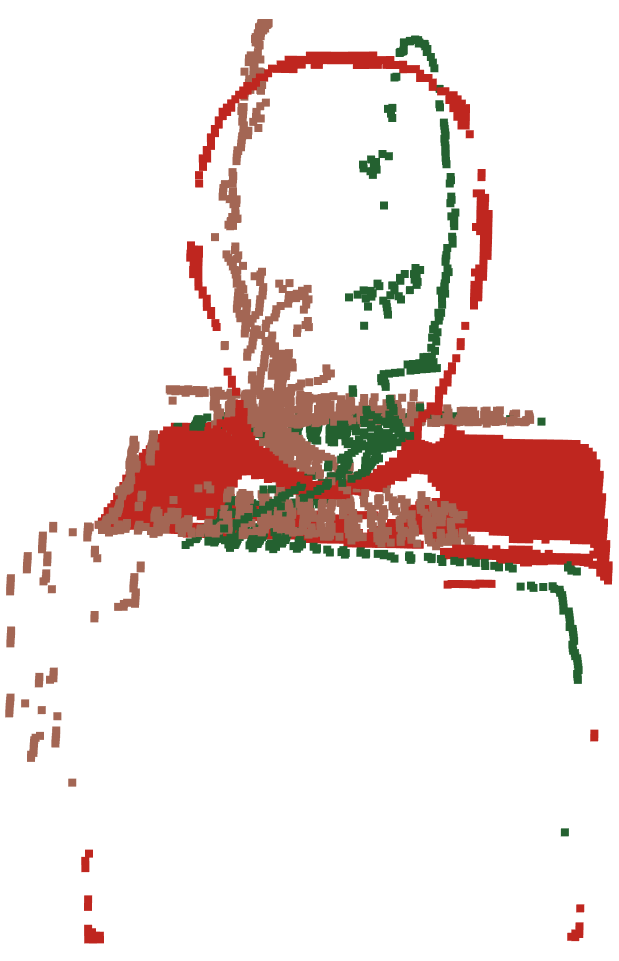
\includegraphics[height=4.9cm]{figures/ror_rem.png}
		\caption{}
		\label{fig:ror:c}
	\end{subfigure}
	\caption{Aplikácia ROR filtrácie s nastaveniami $rad=0.009$ a  $pts=30$: (\textbf{a}) Vstupné mračno bodov vytvorené z IMBM filtrovaných hĺbkových máp. (\textbf{b}) Výstupné mračno bodov po ROR filtrovaní. (\textbf{c}) Odstránené body po ROR filtrácii.}
	\label{fig:ror}
\end{figure}

Na obr. \ref{fig:ror:a}, sa nachádza mračno bodov vytvorené z IMBM filtrovanej hĺbkovej mapy. Výstup ROR filtra, ktorého nastavenia boli $rad=0.009$ a $pts=30$, sa nachádza na obr. \ref{fig:ror:b}. Optimálne nastavenie filtrácie je individuálne pre jednotlivé modely. Grafické prostredie programu umožňuje nastavenie parametrov a vizuálne zobrazenie filtrovaných dát. 

Pri multi-kamerovej kalibrácii sme získali rotačné a translačné parametre pre jednotlivé kamery. Pomocou nich dokážeme dostatočne presne zarovnať filtrované mračná do spoločného priestoru. Presnosť kalibrácie je však ovplyvnená pracovnou teplotou kamery. Jej zmena spôsobuje posun jednotlivých mračien v priestore, čím je ovplyvnená konzistentnosť modelov.

\begin{figure}[h]
	\centering
	\begin{subfigure}[b]{0.32\textwidth}
		\centering
		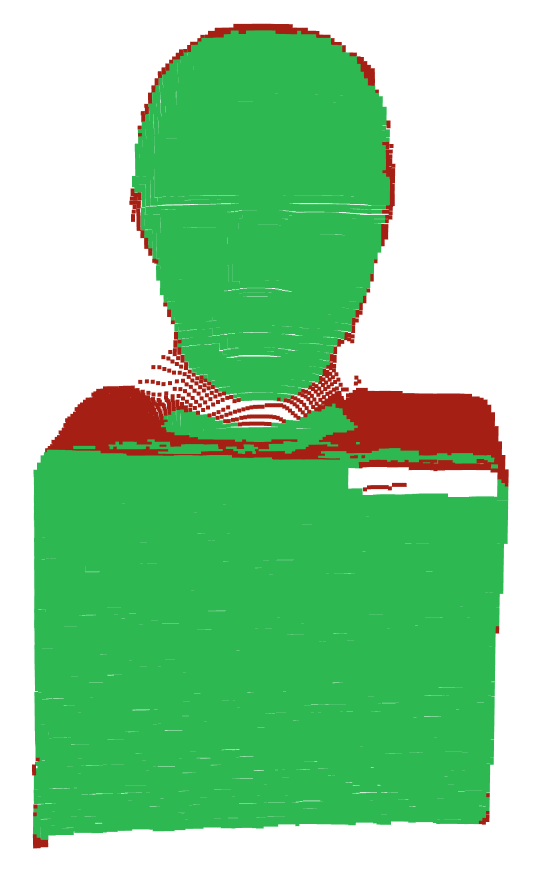
\includegraphics[height=4.5cm]{figures/icp1.png}
		\caption{}
		\label{fig:icp:a}
	\end{subfigure}
	\hfill
	\begin{subfigure}[b]{0.32\textwidth}
		\centering
		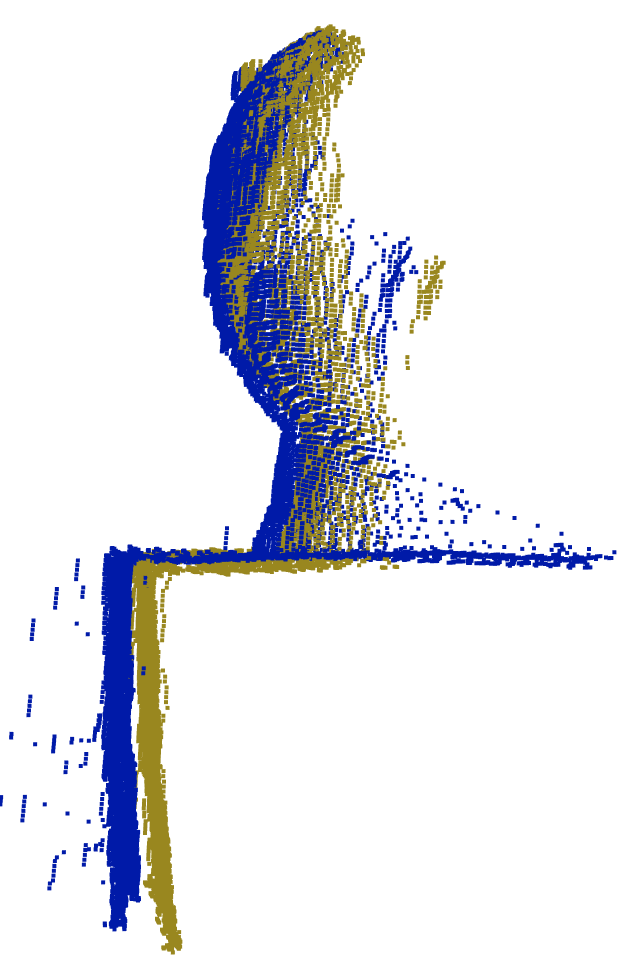
\includegraphics[height=4.5cm]{figures/icp0.png}
		\caption{}
		\label{fig:icp:b}
	\end{subfigure}
	\hfill
	\begin{subfigure}[b]{0.32\textwidth}
		\centering
		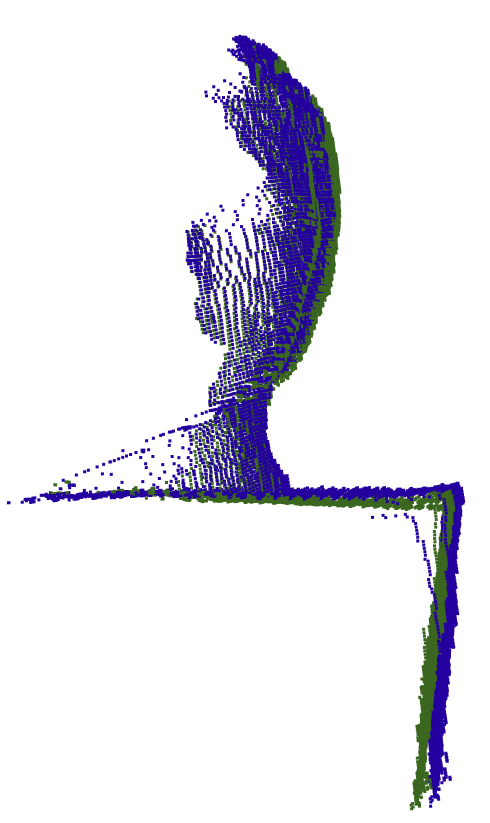
\includegraphics[height=4.5cm]{figures/icp2.png}
		\caption{}
		\label{fig:icp:c}
	\end{subfigure}
	\caption{Zarovnanie mračien pomocou ICP algoritmu: (\textbf{a}) Referenčné mračno bodov, rozdiel medzi nefiltrovaným (červená) a filtrovaným (zelená) mračnom. (\textbf{b}) Rozdiel medzi nezarovnaným nefiltrovaným (modrá) a zarovnaným filtrovaným (žltá) mračnom. (\textbf{c}) Rozdiel medzi nezarovnaným nefiltrovaným (modrá) a zarovnaným filtrovaným (zelená) mračnom.}
	\label{fig:3dm}
\end{figure}

Aplikovaním ICP metódy sa zabezpečí opätovné zarovnanie mračien bodov do spoločného priestoru. Registrácia sa vykonáva postupne medzi dvojicami podvzorkovaných mračien bodov. Predný pohľad tváre je určený ako referenčný a mračno bodov je statické. Rotačná a translačná matica má tvar identickej afinnej transformácie (rovnica \ref{eq_kalib_ident}). Pre ostatné mračná sú vypočítané nové rotačné a translačné parametre zložené z ostatných afinných transformácií. Vstupné nastavenia pre \textit{Incremental registration ICP} \cite{iricp} sú \textit{MaximumIterations}$=20$, \textit{MaxCorrespondenceDistance}$=0,005$ a \textit{RansacOutlierRejectionThreshold}$=0,005$. Zarovnané mračná z jednotlivých kamier sa následne spoja do jedného uceleného mračna. Kvôli vyššej hustote bodov v miestach zarovnania sa v mračne bodov tieto miesta redukujú podľa mriežky (GRID). Týmto sa získa uniformná hustota bodov v celom mračne. 
\begin{figure}[H]
	\centering
	\begin{subfigure}[b]{0.32\textwidth}
		\centering
		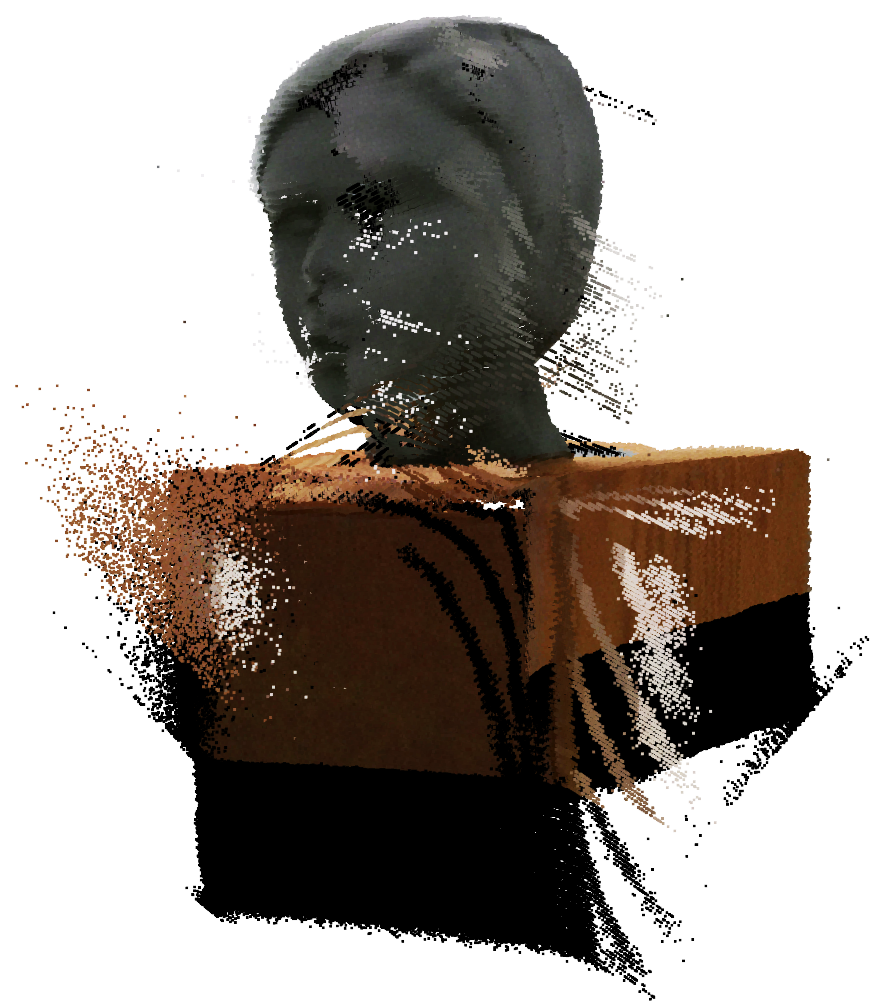
\includegraphics[height=5cm]{figures/model_input.png}
		\caption{}
		\label{fig:model:input}
	\end{subfigure}
	\hfill
	\begin{subfigure}[b]{0.32\textwidth}
		\centering
		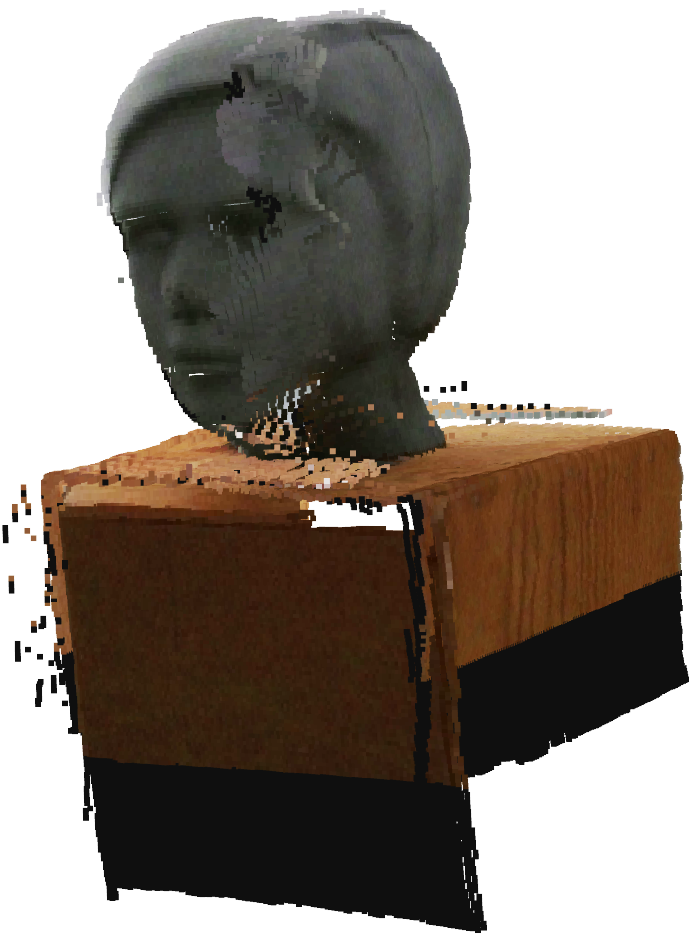
\includegraphics[height=5cm]{figures/model_orig.png}
		\caption{}
		\label{fig:model:imbm}
	\end{subfigure}
	\hfill
	\begin{subfigure}[b]{0.32\textwidth}
		\centering
		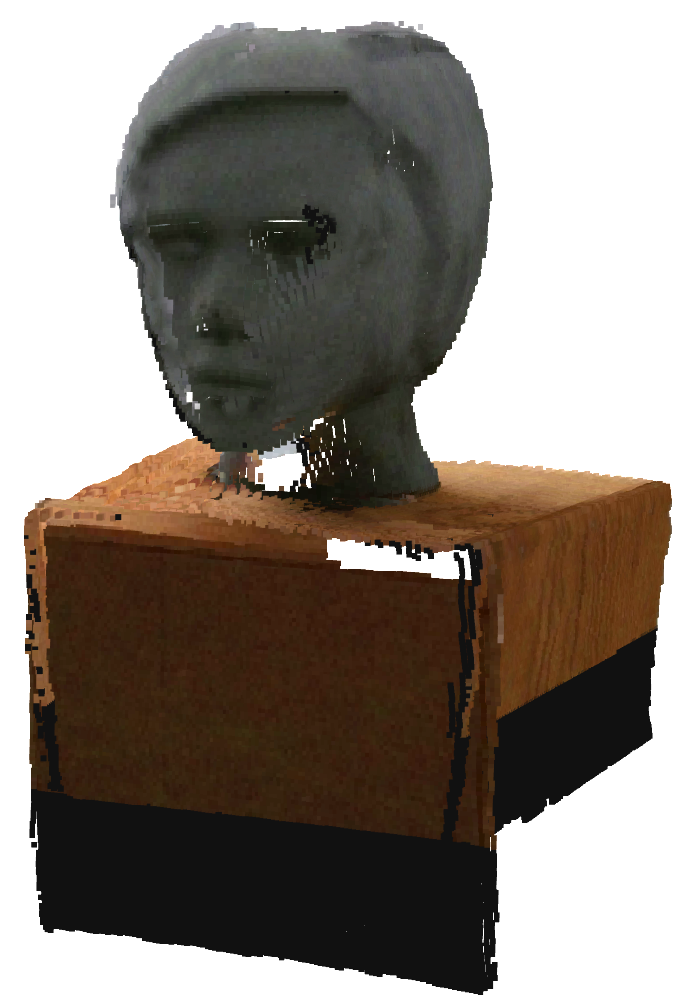
\includegraphics[height=5cm]{figures/model_output.png}
		\caption{}
		\label{fig:model:result}
	\end{subfigure}
	\caption{Proces filtrácie: (\textbf{a}) Mračna bodov získané paralelným snímaním. (\textbf{b}) \, Mračná bodov po IMBM filtrácii. (\textbf{c}) Mračno bodov po ROR + ICP + GRID.}
	\label{fig:model}
\end{figure}


Na obr. \ref{fig:model:input} sa nachádza mračno bodov, ktoré je vytvorené zo série piatich hĺbkových máp zachytených troma ToF kamerami Kinect v2. Snímanie objektu trvalo pod $200ms$. Vplyv multi-kamerovej interferencie je však viditeľný. Na obr. \ref{fig:model:imbm} sa nachádza výstup IMBM filtra, kde je potlačený vplyv multi-kamerovej interferencie. Mračno stále obsahuje šum a lietajúce pixely. Taktiež aj zarovnanie nie je postačujúce. Následným spracovaním pomocou ROR, ICP a GRID sa odstránia chybné pixely a vytvorí sa konzistentné uniformné mračno bodov (obr. \ref{fig:model:result}).


\newpage
\subsection{Automatizované meranie vzdialenosti tvárových čŕt}
Pomocou 68 bodového DLib detektora \cite{king2009dlib} je možné automatizovať meranie určitých parametrov tváre. Jednotlivé merania sú špecifikované v dotazníku využívanom pri vyšetrení na Klinike detí a dorastu
Jesseniovej lekárskej fakulty v Martine, Laboratórium spánkovej medicíny (pozri prílohu \ref{sec:Priloha:Dot}). 
Identifikovaním špecifických kľúčových bodov tváre a prenesením týchto bodov do hĺbkovej mapy je možné pomocou euklidovskej vzdialenosti (rovnica \ref{eq:euclidean}) získať geometrické vlastnosti tvárových parametrov.
Pre meranie OSA bolo vybraných týchto 19 párov kľúčových bodov: 
\vskip 0.2in

\begin{compactitem}
	\item[\textbf{Dĺžka nosa:}] Koreň nosa (28) - Špička nosa (34)
	\item[\textbf{Šírka nosa:}] Ľavá hranica nosa (36) - Pravá hranica nosa (32)
	\item[\textbf{Výška špičky nosa:}] Špička nosa (34) - Horná hranica pery (52)
	\item[\textbf{Šírka ľavého oka:}] Vonkajší kútik oka (46) - Vnútorný kútik oka (43)
	\item[\textbf{Šírka pravého oka:}] Vonkajší kútik oka (37) - Vnútorný kútik oka (40)
	\item[\textbf{Výška pravého oka - 1:}] Vonk. horná kontúra oka (38) - Vonk. dolná kontúra oka (42)
	\item[\textbf{Výška pravého oka - 2:}] Vnut. horná kontúra oka (39) - Vnut. dolná kontúra oka (41)
	\item[\textbf{Výška ľavého oka - 1:}] Vonk. horná kontúra oka (45) - Vonk. dolná kontúra oka (47)
	\item[\textbf{Výška ľavého oka - 2:}] Vnut. horná kontúra oka (44) - Vnut. dolná kontúra oka (48)
	\item[\textbf{Vnútorný rozostup očí:}] Vnút. kútik ľavého oka (43) - Vnút. kútik pravého oka (40)
	\item[\textbf{Vonkajší rozostup očí:}] Vonk. kútik ľavého oka (46) - Vonk. kútik pravého oka (37)
	\item[\textbf{Výška pier:}] Horná hranica pery (52) - Dolná hranica pery (58)
	\item[\textbf{Šírka pier:}] Ľavá hranica pery (55) - Pravá hranica pery (49)
	\item[\textbf{Dĺžka tváre:}] Koreň nosa (28) - Spodná hranica brady (9)
	\item[\textbf{Výška brady:}] Spodná hranica brady (9) - Dolná hranica pery (55)
	\item[\textbf{Dĺžka ľavého spánku:}] Stred ľavého ucha (16) - Vonk. kútik ľavého oka (46)
	\item[\textbf{Dĺžka pravého spánku:}] Stred pravého ucha (2) - Vonk. kútik pravého oka (37)
	\item[\textbf{Dĺžka ľavého líca:}] Stred ľavého ucha (16) - Ľavá hranica pery (55)
	\item[\textbf{Dĺžka pravého líca:}] Stred pravého ucha (2) - Pravá hranica pery (49)
\end{compactitem}

\vskip 0.2in
Meranie bolo vykonané na datasete 270 párov obrazov (RGB-D + hĺbková mapa). Na detekciu kľúčových bodov bol použitý DLib model \textit{shape-predictor-68-face-landmarks}. Každý objekt, ktorý bol použitý pri automatizovanom meraní, mal priradené referenčné hodnoty vzdialenosti pre jednotlivé tvárové parametre. 


Vypočítané hodnoty boli následne porovnané s referenčnými, čím sa získal histogram absolútnej chyby pre všetky merania (Obr. \ref{fig:histogram}). Z celkového počtu 5130 meraní malo 4598 absolútnu chybu menšiu ako 5mm. Zvyšných 532 vykazovalo vyššiu chybu merania nad 10mm. 

\begin{figure}[H]
	\centering
	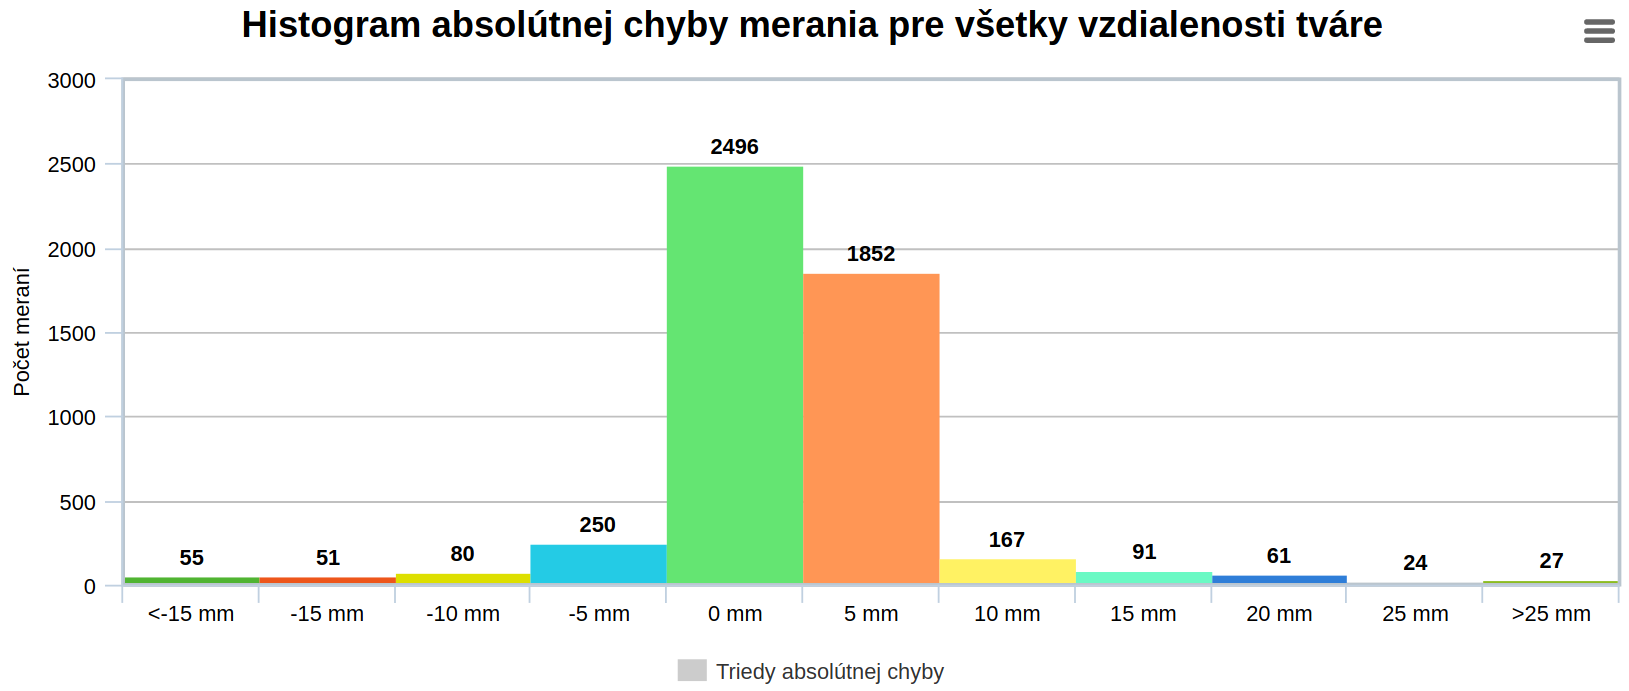
\includegraphics[width=\textwidth]{figures/plot.png}
	\caption{Histogram absolútnej chyby merania tvárových parametrov vytvorený z 5130 meraní euklidovskej vzdialenosti.}
	\label{fig:histogram}
\end{figure}

Vyšší rozdiel medzi referenčnými a nameranými hodnotami môže byť spôsobený zmenou geometrie tváre (zmena mimiky tváre). Takáto chyba sa prejavila napríklad pri výške pier a brady. Problematickými sa javí aj meranie rozmerov spánkov a lícnych častí. 

\begin{figure}[H]
	\centering
	\begin{subfigure}[b]{0.40\textwidth}
		\centering
		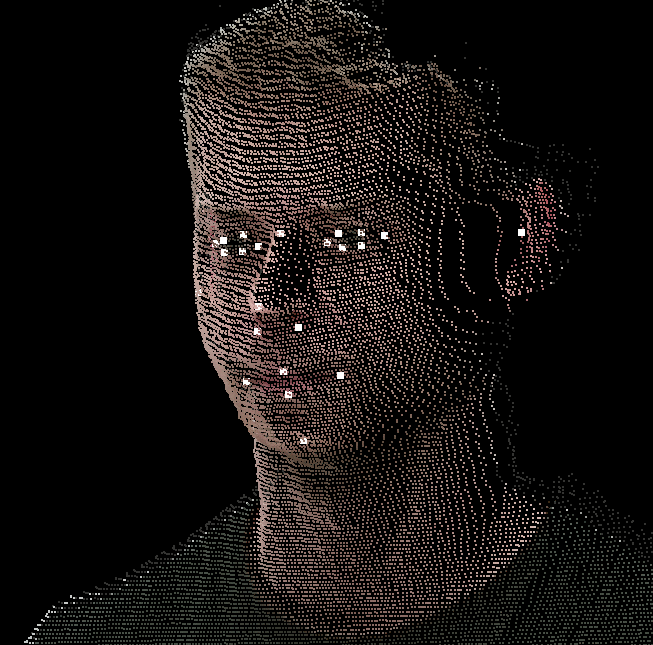
\includegraphics[width=0.9\textwidth]{figures/dlib_cloud_a.png}
		\caption{}
		\label{fig:dlib:cloud:a}
	\end{subfigure}
	\hskip 0.2in
	\begin{subfigure}[b]{0.39\textwidth}
		\centering
		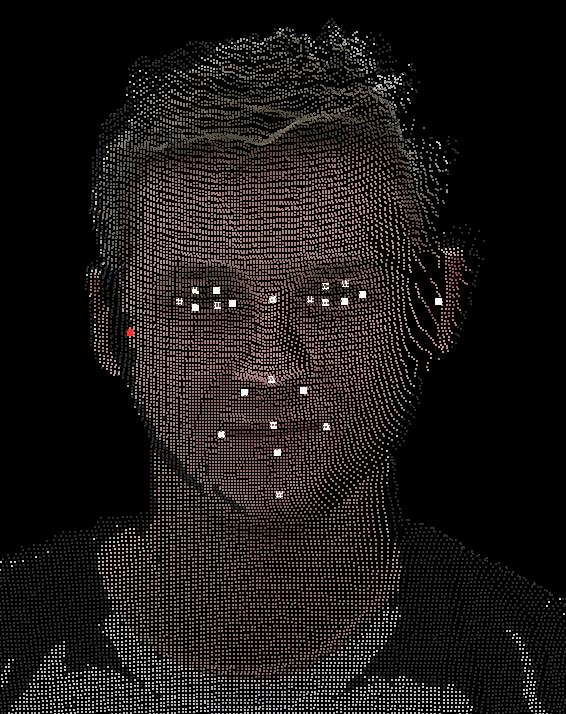
\includegraphics[width=0.7\textwidth]{figures/dlib_cloud_b1.png}
		\caption{}
		\label{fig:dlib:cloud:b}
	\end{subfigure}
	\caption{Ukážka mračna bodov s vyznačenými kľúčovými bodmi: (\textbf{a}) Všetky detekované body boli pod 5mm hranicou absolútnej chyby. (\textbf{b}) Červený bod označuje nepresnú detekciu kľúčového bodu.}
	\label{fig:dlib:cloud}
\end{figure}

Ich príslušné kľúčové parametre sa pri frontálnom pohľade nachádzajú na hranici hĺbkovej mapy. Preto aj pri minimálnej nepresnosti určenia pozície stredov pravého (2) a ľavého ucha (16) môže dôjsť k výraznejšej zmene hĺbky (Obr. \ref{fig:dlib:cloud}). 

Stredné a priemerné hodnoty sú vypočítané z rozdielov výsledných vzdialeností ($d_e-d_e(ref)$). Mínusové hodnoty znamenajú, že automaticky vypočítaná vzdialenosť je menšia ako referenčná.
 
\begin{table}[H]
	\caption{\label{tab:dlib:results} Meranie vybraných faciálnych rozmerov pomocou 68 bodového detektora.}
	\centering
	\begin{tabular}{lccc}
		\toprule
		\textbf{Meranie} & \textbf{Medián [mm]} & \textbf{Average [mm]} & \textbf{Diff (Max-Min) [mm]} \\ 
		\midrule
		\textbf{Dĺžka nosa} 			& 0.19 	& 0.45 	& 9.52	\\
		\textbf{Šírka nosa} 			& 0.12	& -0.27 & 10	\\
		\textbf{Výška špičky nosa} 		& -0.12	& -0.08 & 6.55	\\
		\textbf{Šírka ľavého oka} 		& 0.03	& 0.00	& 7.26	\\
		\textbf{Šírka pravého oka} 		& 0.03 	& 0.09	& 6.90	\\
		\textbf{Výška pravého oka - 1} 	& 0.07	& 0.20	& 12.28	\\
		\textbf{Výška pravého oka - 2} 	& -0.10	& 0.08	& 9.56	\\
		\textbf{Výška ľavého oka - 1} 	& 0.13	& 0.15	& 8.52	\\
		\textbf{Výška ľavého oka - 2} 	& -0.13 & 0.08	& 9.90	\\
		\textbf{Vnútorný rozostup očí} 	& -0.24	& -0.28	& 4.34	\\
		\textbf{Vonkajší rozostup očí} 	& -0.89	& -0.88	& 7.73	\\
		\textbf{Výška pier} 			& 0.77	& 0.42	& 11.47	\\
		\textbf{Šírka pier} 			& -0.19 & 0.04	& 9.07	\\
		\textbf{Dĺžka tváre} 			& -1.82	& -1.81	& 9.28	\\
		\textbf{Výška brady} 			& -3.84	& -3.90	& 11.71	\\
		\textbf{Dĺžka ľavého spánku} 	& 1.47	& 3.06	& \textbf{29.30}	\\
		\textbf{Dĺžka pravého spánku} 	& -10.14& -7.35	& \textbf{90.66}	\\
		\textbf{Dĺžka ľavého líca} 		& -2.07	& -0.80	& \textbf{31.88}	\\
		\textbf{Dĺžka pravého líca} 	& 5.40	& 2.36	& \textbf{69.38}	\\
		\bottomrule
	\end{tabular}
\end{table}

Meranie vzdialeností tvárových parametrov, ktorých kľúčové body sa nenachádzajú na hraniciach hĺbkovej mapy, vykazujú malú absolútnu chybu voči referencii. Problémom je získanie všetkých parametrov z frontálneho pohľadu. Tento problém je však možné vyriešiť dvoma meraniami, kedy poloha tváre pacienta bude vždy mierne natočená. Takéto euklidovské meranie však ukazuje svoje limity pri diagnostike OSA (pozri \ref{sec:med:euclid}). V ďalšej časti sa preto opisuje návrh, ktorý je založený na nových modernejších metódach a môže priniesť lepšie výsledky.

\newpage
\subsection{Segmentácia hĺbkovej mapy}

Pre segmentáciu tvárových častí sa používa hĺbková mapa a RGB-D obraz získaný z IMBM filtra. Pomocou \textit{Mask R-CNN} neurónovej siete dokážeme v RGB-D obraze ohraničiť príslušné tvárové časti \cite{he2017mask}. Následným prenesením identifikovaných regiónov do hĺbkovej mapy vieme konkrétnym pixelom nastaviť klasifikátor, ktorý ich priraďuje do preddefinovaných skupín. 

%Mask R-CNN je rozšírením Faster R-CNN siete a slúži k segmentácii obrazov na úrovni pixelov. Princíp činnosti je znázornený na obr. \ref{fig:mask_rcnn}. Sieť Faster R-CNN  klasifikuje a ohraničuje regióny záujmu (ROI) .V tomto ROI sa následne predpovedajú masky klasifikovaných objektov. Segmentácia na úrovni pixelov vyžaduje jemnejšie zarovnanie, ktoré sa vykonáva cez ROIAlign vrstvu siete. Tá zabezpečuje presnejšie mapovanie masky do pôvodného obrazu. 
%
%\begin{figure}[H]
%	\centering
%	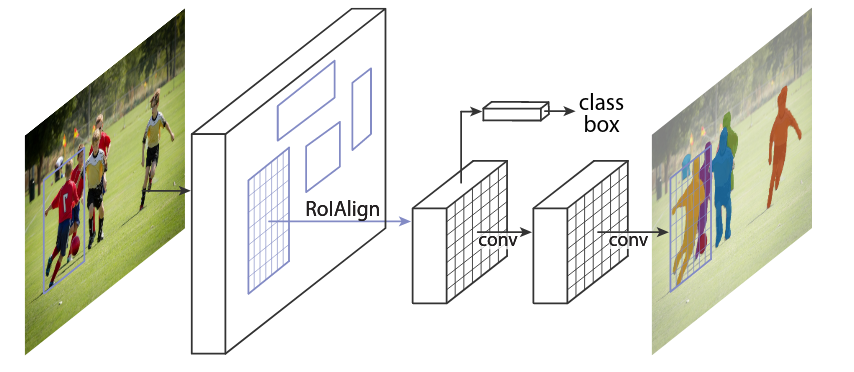
\includegraphics[width=0.75\textwidth]{figures/mask_rcnn.png}
%	\caption{Princíp činnosti neurónovej siete Mask R-CNN .}
%	\label{fig:mask_rcnn}
%\end{figure}

Pre trénovanie tejto siete sme vytvorili dátový set, ktorý pozostával z 65 RGB-D obrazov obsahujúcich 6 rôznych osôb v rozličných polohách. 50 snímok 4 osôb boli použité pre trénovanie a zvyšných 15 obrazov 2 osôb pre testovanie. Vo všetkých obrazoch sa označili regióny prislúchajúce jednotlivým klasifikačným triedam.\newline

\noindent Klasifikované boli tieto oblasti: tvár, nos, ústa, brada, krk, ucho, oko, obočie. 

Vyznačené boli základné časti tváre pomocou nástroja \textit{Via Image Anotator} \cite{dutta2019vgg}. Ukážka RGB-D obrazu s označenými oblasťami sa nachádza v prílohe \ref{fig:mask_label}. Snahou bolo zachytiť tieto oblasti z rôznych uhlov tak, aby boli rozpoznateľné pri použitej multi-kamerovej topológii a pri rôznych pozíciach natočenia hlavy. 

Vychádzali sme z modelu, ktorý už podstúpil trénovanie na ImageNet obrazovom datasete. Tento model bol dotrénovaný na naších dátach. Trénovanie prebiehalo v 60 epochách s  1000 iteráciami. Bola použitá \textit{resnet101} sieťová architektúra. Výsledky trénovania a chyby konkrétnych vrstiev siete sa nachádzajú v tabuľke \ref{tab:rcnn:results}. 

\begin{table}[h]
	\caption{\label{tab:rcnn:results} Vyhodnotenie trénovania Mask R-CNN siete.}
	\centering
	\begin{tabular}{lccc}
		\toprule
		\textbf{Strata} & \textbf{30 epocha} & \textbf{60 epocha} & \textbf{validácia} \\ 
		\midrule
		\textbf{loss} 					& 5,4736 	& 4,579 & 4,698	\\
		\textbf{rpn class loss} 		& 0,6676 	& 0,435 & 0,205	\\
		\textbf{rpn bbox loss} 			& 2,4274	& 2,144 & 2,596	\\
		\textbf{mrcnn class loss} 		& 0,6545	& 0,394 & 0,264	\\
		\textbf{mrcnn bbox loss} 		& 1,0124	& 0,894	& 0,939	\\
		\textbf{mrcnn mask loss} 		& 0,7118	& 0,712	& 0,692	\\
		\bottomrule
	\end{tabular}
\end{table}

Celková stratová funkcia $L$ (\textit{loss}) predstavuje súčet chyby klasifikácie $L_{cls}$ (\textit{class loss}), lokalizácie $L_{box}$ (\textit{bbox loss}) a segmentácie $ L_{mask}$ (\textit{mask loss}). 

\begin{equation}
\label{eq:loss}
\begin{aligned}
L = L_{cls} + L_{box} + L_{mask}
\end{aligned}
\end{equation}

Pre overenie funkčnosti sme klasifikátor použili na nových objektoch. Výsledky segmentácie sa nachádzajú na obr. \ref{fig:rcnn:label}. Z výsledkov segmentácie vidíme, že nie všetky oblasti boli klasifikované.
Niektoré ROI masky boli relatívne dobre segmentované (tvár, nos, ústa). Určíté oblasti však chýbali úplne (oči, krk). Predpokladom je, že rozšírením trénovacieho datasetu o nové RGB-D obrazy sa môže výrazne zvýšiť presnosť klasifikácie a segmentácie. Prenos segmentovaných častí na mračno bodov je znázornené na obr. \ref{fig:rcnn:cloud}.

\begin{figure}[H]
	\centering
	\begin{subfigure}[b]{0.32\textwidth}
		\centering
		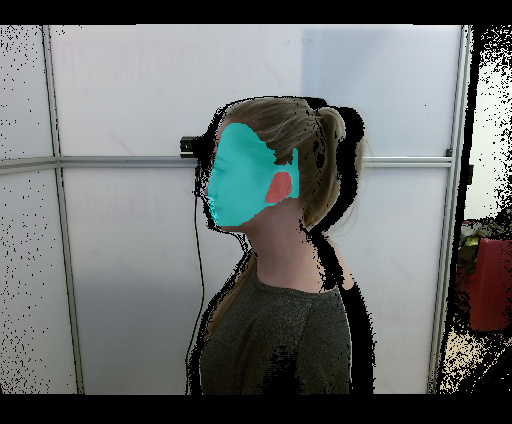
\includegraphics[height=4.3cm]{figures/rcnn_detect1.png}
		\caption{}
		\label{fig:rcnn:label:a}
	\end{subfigure}
	\hskip 0.0in
	\begin{subfigure}[b]{0.32\textwidth}
		\centering
		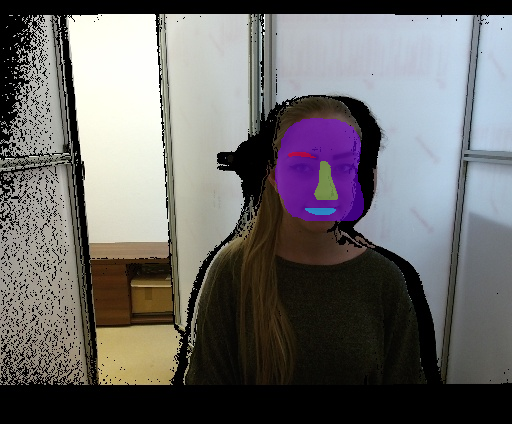
\includegraphics[height=4.3cm]{figures/rcnn_detect2.png}
		\caption{}
		\label{fig:rcnn:label:b}
	\end{subfigure}
	\begin{subfigure}[b]{0.32\textwidth}
		\centering
		\includegraphics[height=4.3cm]{figures/rcnn_detect3.png}
		\caption{}
		\label{fig:rcnn:label:c}
	\end{subfigure}
	\caption{Ukážka segmentácie RGB-D obrazu použitím Mask R-CNN siete: (\textbf{a}) Ľavý pohľad, identifikovaná tvár. (\textbf{b}) Predný pohľad, identifikované obočie, tvár, nos, ústa, brada. (\textbf{c}) Ľavý pohľad, identifikovaná tvár a nos.}
	\label{fig:rcnn:label}
\end{figure}

Výhodou tohto prístupu je, že dokážeme spojiť jednotlivé klasifikované regióny z viacerých pohľadov. Tieto spojené oblasti si navyše uchovávajú aj svoje geometrické vlastnosti (napr. rozostup uší, šírka brady). Pričom pri segmentácii z jednotlivých pohľadov bez spájania do spoločného priestoru by sa táto podstatná informácia strácala. 

\begin{figure}[H]
	\centering
	\includegraphics[width=0.32\textwidth]{figures/rcnn_cloud2.png}
	\caption{Mračno bodov dynamického objektu so zvýraznenými klasifikovanými oblasťami.}
	\label{fig:rcnn:cloud}
\end{figure}

Zlepšenie segmentácie je cieľom budúcej práce. Pre tieto účely bol navrhnutý snímací systém pracujúci s novšími kamerami Intel RealSense d415, ktorý je umiestnený v detskom spánkovom laboratóriu na klinike detí a dorastu v Martine. Ten zabezpečuje zber hĺbkových a RGB-D obrazov pediatrických pacientov z troch perspektív. Spolu s týmito dátami sú ukladané aj informácie o klinickom vyšetrení snímaného pediatrického pacienta (obr. \ref{fig:hmi_web:b} ). Ukážka snímacieho zariadenia sa nachádza na obr \ref{fig:hmi_web:d}. Výstupné dáta budú použité k diagnostike OSA pomocou PointNet2 neurónovej siete \cite{qi2017pointnetplusplus}.

%\begin{figure}[H]
%	\centering
%	\includegraphics[width=\textwidth]{figures/hmi_web1.png}
%	\caption{Zobrazenie webového rozhrania pre zber dát, RGB obraz.}
%	\label{fig:hmi_web:a}
%\end{figure}
%
%\begin{figure}[H]
%	\centering
%	\includegraphics[width=\textwidth]{figures/hmi_web2.png}
%	\caption{Zobrazenie webového rozhranie pre zber dát, hĺbkový obraz.}
%	\label{fig:hmi_web:b}
%\end{figure}


